
% Plantilla para un Trabajo Fin de Grado de la Universidad de Granada,
% adaptada para el Doble Grado en Ingeniería Informática y Matemáticas.
%
%  Autor original de la plantilla original: Mario Román.
%  Enlace: https://github.com/mroman42/templates
%  Cambios en la plantilla por: Javier Sáez
%  Licencia: GNU GPLv2.
%
% Esta plantilla es una adaptación al castellano de la plantilla
% classicthesis de André Miede, que puede obtenerse en:
%  https://ctan.org/tex-archive/macros/latex/contrib/classicthesis?lang=en
% La plantilla original se licencia en GNU GPLv2.
%
% Esta plantilla usa símbolos de la Universidad de Granada sujetos a la normativa
% de identidad visual corporativa, que puede encontrarse en:
% http://secretariageneral.ugr.es/pages/ivc/normativa
%
% La compilación se realiza con las siguientes instrucciones:
%   pdflatex --shell-escape main.tex
%   bibtex main
%   pdflatex --shell-escape main.tex
%   pdflatex --shell-escape main.tex

% Opciones del tipo de documento
\documentclass[oneside,openright,titlepage,numbers=noenddot,openany,headinclude,footinclude=true, cleardoublepage=empty,abstractoff,BCOR=5mm,paper=a4,fontsize=11pt, dvipsnames]{scrreprt}

% LaTeX packages loaded on start
\usepackage[utf8]{inputenc}
\usepackage[T1]{fontenc}
\usepackage{fixltx2e}
\usepackage{graphicx} % Inclusión de imágenes.
\usepackage{grffile}  % Distintos formatos para imágenes.
\usepackage{longtable} % Tablas multipágina.
\usepackage{wrapfig} % Coloca texto alrededor de una figura.
\usepackage{rotating}
\usepackage[normalem]{ulem}
\usepackage{amsmath}
\usepackage{textcomp}
\usepackage{amssymb}
\usepackage{capt-of}
\usepackage[colorlinks=true]{hyperref}
\usepackage{tikz} % Diagramas conmutativos.
\usepackage{minted} % Código fuente.
\usepackage[T1]{fontenc}
\usepackage{natbib}
\usepackage{caption}
\usepackage{ mathrsfs }



\usepackage[toc,page]{appendix}

%% ---------------------- Self added packages
\usepackage{cancel}
\usepackage{cleveref}
\usepackage{bm}

%% ---------------------------------

% Plantilla classicthesis
\usepackage[beramono,eulerchapternumbers,linedheaders,parts,a4paper,dottedtoc,
manychapters,pdfspacing]{classicthesis}

% Geometría y espaciado de párrafos.
\setcounter{secnumdepth}{0}
\usepackage{enumitem}
\setitemize{noitemsep,topsep=0pt,parsep=0pt,partopsep=0pt}
\setlist[enumerate]{topsep=0pt,itemsep=-1ex,partopsep=1ex,parsep=1ex}
\usepackage[top=1in, bottom=1.5in, left=0.9in, right=1.2in]{geometry}
\setlength\itemsep{0em}
\setlength{\parindent}{0pt}
\usepackage{parskip}

% Algoritmos
\usepackage[ruled,vlined]{algorithm2e}
\newcommand\mycommfont[1]{\footnotesize\ttfamily\textcolor{blue}{#1}}
\SetCommentSty{mycommfont}

% Todo notes
\usepackage{todonotes}
\let\marginpar\oldmarginpar

% Profundidad de la tabla de contenidos.
\setcounter{secnumdepth}{3}

% Usa el paquete minted para mostrar trozos de código.
% Pueden seleccionarse el lenguaje apropiado y el estilo del código.
\usepackage{minted}
\usemintedstyle{colorful}
\setminted{fontsize=\small}
\renewcommand{\theFancyVerbLine}{\sffamily\textcolor[rgb]{0.5,0.5,1.0}{\oldstylenums{\arabic{FancyVerbLine}}}}

% Archivos de configuración.
%------------------------
% Math libraries
%------------------------
\usepackage{amsthm}
\usepackage{amsmath}
\usepackage{tikz}
\usepackage{tikz-cd}
\usetikzlibrary{shapes,fit}
\usepackage{bussproofs}
\EnableBpAbbreviations{}
\usepackage{mathtools}
\usepackage{scalerel}
\usepackage{stmaryrd}

%------------------------
% Estilos para los teoremas
%------------------------
\theoremstyle{plain}
\newtheorem{nth}{Theorem}
\newtheorem{nprop}{Proposition}
\newtheorem{lemma}{Lemma}
\newtheorem{corollary}{Corollary}
\theoremstyle{definition}
\newtheorem{ndef}{Definition}
\newtheorem{nproof}{Proof}
\theoremstyle{remark}
\newtheorem{remark}{Remark}
\newtheorem{nexample}{Example}

\begingroup\makeatletter\@for\theoremstyle:=definition,remark,plain\do{\expandafter\g@addto@macro\csname th@\theoremstyle\endcsname{\addtolength\thm@preskip\parskip}}\endgroup

%------------------------
% Macros
% ------------------------

%Frequently used mathematical commands
\newcommand*\diff{\mathop{}\!\mathrm{d}}
\newcommand{\R}{\mathbb{R}}
% \newcommand{\E}{\mathbb{E}}
\newcommand{\bmu}{\bm{\mu}}
\newcommand{\bx}{\bm{x}}
\newcommand{\bX}{\bm{X}}
\newcommand{\bz}{\bm{z}}
\newcommand{\bZ}{\bm{Z}}
\newcommand{\bv}{\bm{v}}
\newcommand{\bh}{\bm{h}}
\newcommand{\bSigma}{\bm{\Sigma}}
\newcommand{\bpi}{\bm{\pi}}
\newcommand{\bLambda}{\bm{\Lambda}}
\newcommand{\btheta}{\bm{\theta}}

\newcommand{\V}{\mathcal{V}}
\newcommand{\D}{\mathcal{D}}
\newcommand{\X}{\mathcal{X}}
\newcommand{\I}{\mathcal{I}}

\newcommand\ddfrac[2]{\frac{\displaystyle #1}{\displaystyle #2}}

\newcommand\E[2]{\mathbb{E}_{#1}\Big[#2\Big]}
\newcommand\KL[2]{KL\Big(#1 \bigm| #2\Big)}
\newcommand{\bigCI}{\mathrel{\text{\scalebox{1.07}{$\perp\mkern-10mu\perp$}}}}
\newcommand{\bigCD}{\centernot{\bigCI}}

\DeclareMathOperator*{\argmax}{arg\,max}
\DeclareMathOperator*{\argmin}{arg\,min}

% My own commands:

\newcommand{\Prob}{\mathcal{P}}
\newcommand{\Alg}{\mathscr{A}}
\newcommand{\N}{\mathbb N}
\newcommand{\A}{\mathcal A}

\newcommand{\abs}[1]{\lvert#1\rvert}  

% Math operators

\DeclareMathOperator*{\Var}{Var}

  % En macros.tex se almacenan las opciones y comandos para escribir matemáticas.
% ****************************************************************************************************
% classicthesis-config.tex 
% formerly known as loadpackages.sty, classicthesis-ldpkg.sty, and classicthesis-preamble.sty 
% Use it at the beginning of your ClassicThesis.tex, or as a LaTeX Preamble 
% in your ClassicThesis.{tex,lyx} with % ****************************************************************************************************
% classicthesis-config.tex 
% formerly known as loadpackages.sty, classicthesis-ldpkg.sty, and classicthesis-preamble.sty 
% Use it at the beginning of your ClassicThesis.tex, or as a LaTeX Preamble 
% in your ClassicThesis.{tex,lyx} with % ****************************************************************************************************
% classicthesis-config.tex 
% formerly known as loadpackages.sty, classicthesis-ldpkg.sty, and classicthesis-preamble.sty 
% Use it at the beginning of your ClassicThesis.tex, or as a LaTeX Preamble 
% in your ClassicThesis.{tex,lyx} with \input{classicthesis-config}
% ****************************************************************************************************  
% If you like the classicthesis, then I would appreciate a postcard. 
% My address can be found in the file ClassicThesis.pdf. A collection 
% of the postcards I received so far is available online at 
% http://postcards.miede.de
% ****************************************************************************************************


% ****************************************************************************************************
% 0. Set the encoding of your files. UTF-8 is the only sensible encoding nowadays. If you can't read
% äöüßáéçèê∂åëæƒÏ€ then change the encoding setting in your editor, not the line below. If your editor
% does not support utf8 use another editor!
% ****************************************************************************************************
\PassOptionsToPackage{utf8x}{inputenc}
	\usepackage{inputenc}

% ****************************************************************************************************
% 1. Configure classicthesis for your needs here, e.g., remove "drafting" below 
% in order to deactivate the time-stamp on the pages
% ****************************************************************************************************
%Old
%\PassOptionsToPackage{eulerchapternumbers,listings,drafting,%
%		pdfspacing,%floatperchapter,%linedheaders,%
%                subfig,beramono,eulermath,parts,dottedtoc}{classicthesis}                                        
% ********************************************************************
% Arsclassica , another template
\usepackage{arsclassica}
\PassOptionsToPackage{
  drafting=true,    % print version information on the bottom of the pages
  tocaligned=false, % the left column of the toc will be aligned (no indentation)
  dottedtoc=false,  % page numbers in ToC flushed right
  eulerchapternumbers=true, % use AMS Euler for chapter font (otherwise Palatino)
  linedheaders=false,       % chaper headers will have line above and beneath
  floatperchapter=true,     % numbering per chapter for all floats (i.e., Figure 1.1)
  eulermath=true,  % use awesome Euler fonts for mathematical formulae (only with pdfLaTeX)
  beramono=true,    % toggle a nice monospaced font (w/ bold)
  iosevka=true,
  palatino=true,    % deactivate standard font for loading another one, see the last section at the end of this file for suggestions
  style=arsclassica % classicthesis, arsclassica
}{classicthesis}


%\newcommand*{\Chapter}[1]{%
%
%	\chapter{}%[#1: \textit{#2}]{#1}%
%    \begingroup
%    \raggedright\Large
%    \spacedallcaps{#1}\par
%    \endgroup
%    \nobreak\vspace{\glueexpr \bigskipamount*3 \relax}%
%    % Adjust this factor as needed ..........^
%}

\renewcommand\formatchapter[1]{%
    \setbox0\hbox{\chapterNumber\thechapter\hspace{10pt}\ \\ }%
    \begin{minipage}[t]{\dimexpr\linewidth-\wd0\relax}%
    \raggedright\spacedallcaps{#1}%
    \end{minipage}%
}






% Available options for classicthesis.sty 
% (see ClassicThesis.pdf for more information):
% drafting
% parts nochapters linedheaders
% eulerchapternumbers beramono eulermath pdfspacing minionprospacing
% tocaligned dottedtoc manychapters
% listings floatperchapter subfig
% ********************************************************************

% ****************************************************************************************************
% 2. Personal data and user ad-hoc commands
% ****************************************************************************************************
\newcommand{\myTitle}{A Classic Thesis Style\xspace}
\newcommand{\mySubtitle}{An Homage to The Elements of Typographic Style\xspace}
\newcommand{\myDegree}{Doktor-Ingenieur (Dr.-Ing.)\xspace}
\newcommand{\myName}{André Miede\xspace}
\newcommand{\myProf}{Put name here\xspace}
\newcommand{\myOtherProf}{Put name here\xspace}
\newcommand{\mySupervisor}{Put name here\xspace}
\newcommand{\myFaculty}{Put data here\xspace}
\newcommand{\myDepartment}{Put data here\xspace}
\newcommand{\myUni}{Put data here\xspace}
\newcommand{\myLocation}{Saarbrücken\xspace}
\newcommand{\myTime}{September 2015\xspace}
%\newcommand{\myVersion}{version 4.2\xspace}

% ********************************************************************
% Setup, finetuning, and useful commands
% ********************************************************************
\newcounter{dummy} % necessary for correct hyperlinks (to index, bib, etc.)
\newlength{\abcd} % for ab..z string length calculation
\providecommand{\mLyX}{L\kern-.1667em\lower.25em\hbox{Y}\kern-.125emX\@}
\newcommand{\ie}{i.\,e.}
\newcommand{\Ie}{I.\,e.}
\newcommand{\eg}{e.\,g.}
\newcommand{\Eg}{E.\,g.} 
% ****************************************************************************************************


% ****************************************************************************************************
% 3. Loading some handy packages
% ****************************************************************************************************
% ******************************************************************** 
% Packages with options that might require adjustments
% ******************************************************************** 
%\PassOptionsToPackage{ngerman,american}{babel}   % change this to your language(s)
% Spanish languages need extra options in order to work with this template
% \PassOptionsToPackage{es-lcroman,spanish}{babel}
\usepackage[main=english]{babel}

%\usepackage{csquotes}
% \PassOptionsToPackage{%
%     %backend=biber, %instead of bibtex
% 	backend=bibtex8,bibencoding=ascii,%
% 	language=auto,%
% 	style=alpha,%
%     %style=authoryear-comp, % Author 1999, 2010
%     %bibstyle=authoryear,dashed=false, % dashed: substitute rep. author with ---
%     sorting=nyt, % name, year, title
%     maxbibnames=10, % default: 3, et al.
%     %backref=true,%
%     natbib=true % natbib compatibility mode (\citep and \citet still work)
% }{biblatex}
%     \usepackage{biblatex}

% \PassOptionsToPackage{fleqn}{amsmath}       % math environments and more by the AMS 
%     \usepackage{amsmath}

% ******************************************************************** 
% General useful packages
% ******************************************************************** 
\PassOptionsToPackage{T1}{fontenc} % T2A for cyrillics
    \usepackage{fontenc}     
\usepackage{textcomp} % fix warning with missing font shapes
\usepackage{scrhack} % fix warnings when using KOMA with listings package          
\usepackage{xspace} % to get the spacing after macros right  
\usepackage{mparhack} % get marginpar right
\usepackage{fixltx2e} % fixes some LaTeX stuff --> since 2015 in the LaTeX kernel (see below)
%\usepackage[latest]{latexrelease} % will be used once available in more distributions (ISSUE #107)
\PassOptionsToPackage{printonlyused,smaller}{acronym} 
    \usepackage{acronym} % nice macros for handling all acronyms in the thesis
    %\renewcommand{\bflabel}[1]{{#1}\hfill} % fix the list of acronyms --> no longer working
    %\renewcommand*{\acsfont}[1]{\textsc{#1}} 
    \renewcommand*{\aclabelfont}[1]{\acsfont{#1}}
% ****************************************************************************************************


% ****************************************************************************************************
% 4. Setup floats: tables, (sub)figures, and captions
% ****************************************************************************************************
\usepackage{tabularx} % better tables
    \setlength{\extrarowheight}{3pt} % increase table row height
\newcommand{\tableheadline}[1]{\multicolumn{1}{c}{\spacedlowsmallcaps{#1}}}
\newcommand{\myfloatalign}{\centering} % to be used with each float for alignment
\usepackage{caption}
% Thanks to cgnieder and Claus Lahiri
% http://tex.stackexchange.com/questions/69349/spacedlowsmallcaps-in-caption-label
% [REMOVED DUE TO OTHER PROBLEMS, SEE ISSUE #82]    
%\DeclareCaptionLabelFormat{smallcaps}{\bothIfFirst{#1}{~}\MakeTextLowercase{\textsc{#2}}}
%\captionsetup{font=small,labelformat=smallcaps} % format=hang,
\captionsetup{font=small} % format=hang,
\usepackage{subfig}  
% ****************************************************************************************************


% ****************************************************************************************************
% 5. Setup code listings
% ****************************************************************************************************
% \usepackage{listings} 
% %\lstset{emph={trueIndex,root},emphstyle=\color{BlueViolet}}%\underbar} % for special keywords
% \lstset{language={Haskell},morekeywords={PassOptionsToPackage,selectlanguage},keywordstyle=\color{RoyalBlue},basicstyle=\small\ttfamily,commentstyle=\color{Green}\ttfamily,stringstyle=\rmfamily,numbers=none,numberstyle=\scriptsize,stepnumber=5,numbersep=8pt,showstringspaces=false,breaklines=true,belowcaptionskip=.75\baselineskip} 
% ****************************************************************************************************             


% ****************************************************************************************************
% 6. PDFLaTeX, hyperreferences and citation backreferences
% ****************************************************************************************************
% ********************************************************************
% Using PDFLaTeX
% ********************************************************************
\PassOptionsToPackage{pdftex,hyperfootnotes=false,pdfpagelabels}{hyperref}
    \usepackage{hyperref}  % backref linktocpage pagebackref
\pdfcompresslevel=9
\pdfadjustspacing=1 
\PassOptionsToPackage{pdftex}{graphicx}
    \usepackage{graphicx} 
 

% ********************************************************************
% Hyperreferences
% ********************************************************************
\hypersetup{%
    %draft, % = no hyperlinking at all (useful in b/w printouts)
    colorlinks=true, linktocpage=true, pdfstartpage=3, pdfstartview=FitV,%
    % uncomment the following line if you want to have black links (e.g., for printing)
    %colorlinks=false, linktocpage=false, pdfstartpage=3, pdfstartview=FitV, pdfborder={0 0 0},%
    breaklinks=true, pdfpagemode=UseNone, pageanchor=true, pdfpagemode=UseOutlines,%
    plainpages=false, bookmarksnumbered, bookmarksopen=true, bookmarksopenlevel=1,%
    hypertexnames=true, pdfhighlight=/O,%nesting=true,%frenchlinks,%
    urlcolor=webbrown, linkcolor=RoyalBlue, citecolor=webgreen, %pagecolor=RoyalBlue,%
    %urlcolor=Black, linkcolor=Black, citecolor=Black, %pagecolor=Black,%
    pdftitle={\myTitle},%
    pdfauthor={\textcopyright\ \myName, \myUni, \myFaculty},%
    pdfsubject={},%
    pdfkeywords={},%
    pdfcreator={pdfLaTeX},%
    pdfproducer={LaTeX with hyperref and classicthesis}%
}   

% ********************************************************************
% Setup autoreferences
% ********************************************************************
% There are some issues regarding autorefnames
% http://www.ureader.de/msg/136221647.aspx
% http://www.tex.ac.uk/cgi-bin/texfaq2html?label=latexwords
% you have to redefine the makros for the 
% language you use, e.g., american, ngerman
% (as chosen when loading babel/AtBeginDocument)
% ********************************************************************
\makeatletter
\@ifpackageloaded{babel}%
    {%
       \addto\extrasamerican{%
			\renewcommand*{\figureautorefname}{Figure}%
			\renewcommand*{\tableautorefname}{Table}%
			\renewcommand*{\partautorefname}{Part}%
			\renewcommand*{\chapterautorefname}{Chapter}%
			\renewcommand*{\sectionautorefname}{Section}%
			\renewcommand*{\subsectionautorefname}{Section}%
			\renewcommand*{\subsubsectionautorefname}{Section}%     
                }%
       \addto\extrasngerman{% 
			\renewcommand*{\paragraphautorefname}{Absatz}%
			\renewcommand*{\subparagraphautorefname}{Unterabsatz}%
			\renewcommand*{\footnoteautorefname}{Fu\"snote}%
			\renewcommand*{\FancyVerbLineautorefname}{Zeile}%
			\renewcommand*{\theoremautorefname}{Theorem}%
			\renewcommand*{\appendixautorefname}{Anhang}%
			\renewcommand*{\equationautorefname}{Gleichung}%        
			\renewcommand*{\itemautorefname}{Punkt}%
                }%  
            % Fix to getting autorefs for subfigures right (thanks to Belinda Vogt for changing the definition)
            \providecommand{\subfigureautorefname}{\figureautorefname}%             
    }{\relax}
\makeatother

% ************************************************************ 
% This needs to be done after classicthesis includes xcolor
% and hyperref
% ************************************************************

\usepackage{amsthm}
\usepackage{parskip}
%\usepackage{pgfplots}
%\pgfplotsset{compat=1.17}

\usepackage[theorems, skins, breakable]{tcolorbox}
\tcolorboxenvironment{ndef}{
	blanker,
	breakable,
	left=12pt,
	%before skip=12pt,
	after skip=12pt,
	borderline west={2pt}{0pt}{gray},
	before upper={\parindent 12pt}
}

\tcolorboxenvironment{nprop}{
	blanker,
	breakable,
	left=12pt,
	%before skip=12pt,
	after skip=12pt,
	borderline west={2pt}{0pt}{gray},
	before upper={\parindent 12pt}
}

\tcolorboxenvironment{corollary}{
	blanker,
	breakable,
	left=12pt,
	%before skip=12pt,
	after skip=12pt,
	borderline west={2pt}{0pt}{gray},
	before upper={\parindent 12pt}
}

\tcolorboxenvironment{nth}{
	blanker,
	breakable,
	left=12pt,
	%before skip=12pt,
	after skip=12pt,
	borderline west={2pt}{0pt}{gray},
	before upper={\parindent 12pt}
}

% ****************************************************************************************************
% 7. Last calls before the bar closes
% ****************************************************************************************************
% ********************************************************************
% Development Stuff
% ********************************************************************
\listfiles
%\PassOptionsToPackage{l2tabu,orthodox,abort}{nag}
%   \usepackage{nag}
%\PassOptionsToPackage{warning, all}{onlyamsmath}
%   \usepackage{onlyamsmath}

% ********************************************************************
% Last, but not least...
% ********************************************************************
\usepackage{classicthesis} 
% ****************************************************************************************************


% ****************************************************************************************************
% 8. Further adjustments (experimental)
% ****************************************************************************************************
% ********************************************************************
% Changing the text area
% ********************************************************************
\linespread{1.05} % a bit more for Palatino
% \areaset[current]{325pt}{680pt} % 686 (factor 2.2) + 33 head + 42 head \the\footskip
%\setlength{\marginparwidth}{7em}%
%\setlength{\marginparsep}{2em}%

% ********************************************************************
% Using different fonts
% ********************************************************************
%\usepackage[oldstylenums]{kpfonts} % oldstyle notextcomp
%\usepackage[osf]{libertine}
%\usepackage[light,condensed,math]{iwona}
%\renewcommand{\sfdefault}{iwona}
%\usepackage{lmodern} % <-- no osf support :-(
%\usepackage{cfr-lm} % 
%\usepackage[urw-garamond]{mathdesign}% <-- no osf support :-(
%\usepackage[default,osfigures]{opensans} % scale=0.95 
%\usepackage[sfdefault]{FiraSans}
% ****************************************************************************************************
% ****************************************************************************************************  
% If you like the classicthesis, then I would appreciate a postcard. 
% My address can be found in the file ClassicThesis.pdf. A collection 
% of the postcards I received so far is available online at 
% http://postcards.miede.de
% ****************************************************************************************************


% ****************************************************************************************************
% 0. Set the encoding of your files. UTF-8 is the only sensible encoding nowadays. If you can't read
% äöüßáéçèê∂åëæƒÏ€ then change the encoding setting in your editor, not the line below. If your editor
% does not support utf8 use another editor!
% ****************************************************************************************************
\PassOptionsToPackage{utf8x}{inputenc}
	\usepackage{inputenc}

% ****************************************************************************************************
% 1. Configure classicthesis for your needs here, e.g., remove "drafting" below 
% in order to deactivate the time-stamp on the pages
% ****************************************************************************************************
%Old
%\PassOptionsToPackage{eulerchapternumbers,listings,drafting,%
%		pdfspacing,%floatperchapter,%linedheaders,%
%                subfig,beramono,eulermath,parts,dottedtoc}{classicthesis}                                        
% ********************************************************************
% Arsclassica , another template
\usepackage{arsclassica}
\PassOptionsToPackage{
  drafting=true,    % print version information on the bottom of the pages
  tocaligned=false, % the left column of the toc will be aligned (no indentation)
  dottedtoc=false,  % page numbers in ToC flushed right
  eulerchapternumbers=true, % use AMS Euler for chapter font (otherwise Palatino)
  linedheaders=false,       % chaper headers will have line above and beneath
  floatperchapter=true,     % numbering per chapter for all floats (i.e., Figure 1.1)
  eulermath=true,  % use awesome Euler fonts for mathematical formulae (only with pdfLaTeX)
  beramono=true,    % toggle a nice monospaced font (w/ bold)
  iosevka=true,
  palatino=true,    % deactivate standard font for loading another one, see the last section at the end of this file for suggestions
  style=arsclassica % classicthesis, arsclassica
}{classicthesis}


%\newcommand*{\Chapter}[1]{%
%
%	\chapter{}%[#1: \textit{#2}]{#1}%
%    \begingroup
%    \raggedright\Large
%    \spacedallcaps{#1}\par
%    \endgroup
%    \nobreak\vspace{\glueexpr \bigskipamount*3 \relax}%
%    % Adjust this factor as needed ..........^
%}

\renewcommand\formatchapter[1]{%
    \setbox0\hbox{\chapterNumber\thechapter\hspace{10pt}\ \\ }%
    \begin{minipage}[t]{\dimexpr\linewidth-\wd0\relax}%
    \raggedright\spacedallcaps{#1}%
    \end{minipage}%
}






% Available options for classicthesis.sty 
% (see ClassicThesis.pdf for more information):
% drafting
% parts nochapters linedheaders
% eulerchapternumbers beramono eulermath pdfspacing minionprospacing
% tocaligned dottedtoc manychapters
% listings floatperchapter subfig
% ********************************************************************

% ****************************************************************************************************
% 2. Personal data and user ad-hoc commands
% ****************************************************************************************************
\newcommand{\myTitle}{A Classic Thesis Style\xspace}
\newcommand{\mySubtitle}{An Homage to The Elements of Typographic Style\xspace}
\newcommand{\myDegree}{Doktor-Ingenieur (Dr.-Ing.)\xspace}
\newcommand{\myName}{André Miede\xspace}
\newcommand{\myProf}{Put name here\xspace}
\newcommand{\myOtherProf}{Put name here\xspace}
\newcommand{\mySupervisor}{Put name here\xspace}
\newcommand{\myFaculty}{Put data here\xspace}
\newcommand{\myDepartment}{Put data here\xspace}
\newcommand{\myUni}{Put data here\xspace}
\newcommand{\myLocation}{Saarbrücken\xspace}
\newcommand{\myTime}{September 2015\xspace}
%\newcommand{\myVersion}{version 4.2\xspace}

% ********************************************************************
% Setup, finetuning, and useful commands
% ********************************************************************
\newcounter{dummy} % necessary for correct hyperlinks (to index, bib, etc.)
\newlength{\abcd} % for ab..z string length calculation
\providecommand{\mLyX}{L\kern-.1667em\lower.25em\hbox{Y}\kern-.125emX\@}
\newcommand{\ie}{i.\,e.}
\newcommand{\Ie}{I.\,e.}
\newcommand{\eg}{e.\,g.}
\newcommand{\Eg}{E.\,g.} 
% ****************************************************************************************************


% ****************************************************************************************************
% 3. Loading some handy packages
% ****************************************************************************************************
% ******************************************************************** 
% Packages with options that might require adjustments
% ******************************************************************** 
%\PassOptionsToPackage{ngerman,american}{babel}   % change this to your language(s)
% Spanish languages need extra options in order to work with this template
% \PassOptionsToPackage{es-lcroman,spanish}{babel}
\usepackage[main=english]{babel}

%\usepackage{csquotes}
% \PassOptionsToPackage{%
%     %backend=biber, %instead of bibtex
% 	backend=bibtex8,bibencoding=ascii,%
% 	language=auto,%
% 	style=alpha,%
%     %style=authoryear-comp, % Author 1999, 2010
%     %bibstyle=authoryear,dashed=false, % dashed: substitute rep. author with ---
%     sorting=nyt, % name, year, title
%     maxbibnames=10, % default: 3, et al.
%     %backref=true,%
%     natbib=true % natbib compatibility mode (\citep and \citet still work)
% }{biblatex}
%     \usepackage{biblatex}

% \PassOptionsToPackage{fleqn}{amsmath}       % math environments and more by the AMS 
%     \usepackage{amsmath}

% ******************************************************************** 
% General useful packages
% ******************************************************************** 
\PassOptionsToPackage{T1}{fontenc} % T2A for cyrillics
    \usepackage{fontenc}     
\usepackage{textcomp} % fix warning with missing font shapes
\usepackage{scrhack} % fix warnings when using KOMA with listings package          
\usepackage{xspace} % to get the spacing after macros right  
\usepackage{mparhack} % get marginpar right
\usepackage{fixltx2e} % fixes some LaTeX stuff --> since 2015 in the LaTeX kernel (see below)
%\usepackage[latest]{latexrelease} % will be used once available in more distributions (ISSUE #107)
\PassOptionsToPackage{printonlyused,smaller}{acronym} 
    \usepackage{acronym} % nice macros for handling all acronyms in the thesis
    %\renewcommand{\bflabel}[1]{{#1}\hfill} % fix the list of acronyms --> no longer working
    %\renewcommand*{\acsfont}[1]{\textsc{#1}} 
    \renewcommand*{\aclabelfont}[1]{\acsfont{#1}}
% ****************************************************************************************************


% ****************************************************************************************************
% 4. Setup floats: tables, (sub)figures, and captions
% ****************************************************************************************************
\usepackage{tabularx} % better tables
    \setlength{\extrarowheight}{3pt} % increase table row height
\newcommand{\tableheadline}[1]{\multicolumn{1}{c}{\spacedlowsmallcaps{#1}}}
\newcommand{\myfloatalign}{\centering} % to be used with each float for alignment
\usepackage{caption}
% Thanks to cgnieder and Claus Lahiri
% http://tex.stackexchange.com/questions/69349/spacedlowsmallcaps-in-caption-label
% [REMOVED DUE TO OTHER PROBLEMS, SEE ISSUE #82]    
%\DeclareCaptionLabelFormat{smallcaps}{\bothIfFirst{#1}{~}\MakeTextLowercase{\textsc{#2}}}
%\captionsetup{font=small,labelformat=smallcaps} % format=hang,
\captionsetup{font=small} % format=hang,
\usepackage{subfig}  
% ****************************************************************************************************


% ****************************************************************************************************
% 5. Setup code listings
% ****************************************************************************************************
% \usepackage{listings} 
% %\lstset{emph={trueIndex,root},emphstyle=\color{BlueViolet}}%\underbar} % for special keywords
% \lstset{language={Haskell},morekeywords={PassOptionsToPackage,selectlanguage},keywordstyle=\color{RoyalBlue},basicstyle=\small\ttfamily,commentstyle=\color{Green}\ttfamily,stringstyle=\rmfamily,numbers=none,numberstyle=\scriptsize,stepnumber=5,numbersep=8pt,showstringspaces=false,breaklines=true,belowcaptionskip=.75\baselineskip} 
% ****************************************************************************************************             


% ****************************************************************************************************
% 6. PDFLaTeX, hyperreferences and citation backreferences
% ****************************************************************************************************
% ********************************************************************
% Using PDFLaTeX
% ********************************************************************
\PassOptionsToPackage{pdftex,hyperfootnotes=false,pdfpagelabels}{hyperref}
    \usepackage{hyperref}  % backref linktocpage pagebackref
\pdfcompresslevel=9
\pdfadjustspacing=1 
\PassOptionsToPackage{pdftex}{graphicx}
    \usepackage{graphicx} 
 

% ********************************************************************
% Hyperreferences
% ********************************************************************
\hypersetup{%
    %draft, % = no hyperlinking at all (useful in b/w printouts)
    colorlinks=true, linktocpage=true, pdfstartpage=3, pdfstartview=FitV,%
    % uncomment the following line if you want to have black links (e.g., for printing)
    %colorlinks=false, linktocpage=false, pdfstartpage=3, pdfstartview=FitV, pdfborder={0 0 0},%
    breaklinks=true, pdfpagemode=UseNone, pageanchor=true, pdfpagemode=UseOutlines,%
    plainpages=false, bookmarksnumbered, bookmarksopen=true, bookmarksopenlevel=1,%
    hypertexnames=true, pdfhighlight=/O,%nesting=true,%frenchlinks,%
    urlcolor=webbrown, linkcolor=RoyalBlue, citecolor=webgreen, %pagecolor=RoyalBlue,%
    %urlcolor=Black, linkcolor=Black, citecolor=Black, %pagecolor=Black,%
    pdftitle={\myTitle},%
    pdfauthor={\textcopyright\ \myName, \myUni, \myFaculty},%
    pdfsubject={},%
    pdfkeywords={},%
    pdfcreator={pdfLaTeX},%
    pdfproducer={LaTeX with hyperref and classicthesis}%
}   

% ********************************************************************
% Setup autoreferences
% ********************************************************************
% There are some issues regarding autorefnames
% http://www.ureader.de/msg/136221647.aspx
% http://www.tex.ac.uk/cgi-bin/texfaq2html?label=latexwords
% you have to redefine the makros for the 
% language you use, e.g., american, ngerman
% (as chosen when loading babel/AtBeginDocument)
% ********************************************************************
\makeatletter
\@ifpackageloaded{babel}%
    {%
       \addto\extrasamerican{%
			\renewcommand*{\figureautorefname}{Figure}%
			\renewcommand*{\tableautorefname}{Table}%
			\renewcommand*{\partautorefname}{Part}%
			\renewcommand*{\chapterautorefname}{Chapter}%
			\renewcommand*{\sectionautorefname}{Section}%
			\renewcommand*{\subsectionautorefname}{Section}%
			\renewcommand*{\subsubsectionautorefname}{Section}%     
                }%
       \addto\extrasngerman{% 
			\renewcommand*{\paragraphautorefname}{Absatz}%
			\renewcommand*{\subparagraphautorefname}{Unterabsatz}%
			\renewcommand*{\footnoteautorefname}{Fu\"snote}%
			\renewcommand*{\FancyVerbLineautorefname}{Zeile}%
			\renewcommand*{\theoremautorefname}{Theorem}%
			\renewcommand*{\appendixautorefname}{Anhang}%
			\renewcommand*{\equationautorefname}{Gleichung}%        
			\renewcommand*{\itemautorefname}{Punkt}%
                }%  
            % Fix to getting autorefs for subfigures right (thanks to Belinda Vogt for changing the definition)
            \providecommand{\subfigureautorefname}{\figureautorefname}%             
    }{\relax}
\makeatother

% ************************************************************ 
% This needs to be done after classicthesis includes xcolor
% and hyperref
% ************************************************************

\usepackage{amsthm}
\usepackage{parskip}
%\usepackage{pgfplots}
%\pgfplotsset{compat=1.17}

\usepackage[theorems, skins, breakable]{tcolorbox}
\tcolorboxenvironment{ndef}{
	blanker,
	breakable,
	left=12pt,
	%before skip=12pt,
	after skip=12pt,
	borderline west={2pt}{0pt}{gray},
	before upper={\parindent 12pt}
}

\tcolorboxenvironment{nprop}{
	blanker,
	breakable,
	left=12pt,
	%before skip=12pt,
	after skip=12pt,
	borderline west={2pt}{0pt}{gray},
	before upper={\parindent 12pt}
}

\tcolorboxenvironment{corollary}{
	blanker,
	breakable,
	left=12pt,
	%before skip=12pt,
	after skip=12pt,
	borderline west={2pt}{0pt}{gray},
	before upper={\parindent 12pt}
}

\tcolorboxenvironment{nth}{
	blanker,
	breakable,
	left=12pt,
	%before skip=12pt,
	after skip=12pt,
	borderline west={2pt}{0pt}{gray},
	before upper={\parindent 12pt}
}

% ****************************************************************************************************
% 7. Last calls before the bar closes
% ****************************************************************************************************
% ********************************************************************
% Development Stuff
% ********************************************************************
\listfiles
%\PassOptionsToPackage{l2tabu,orthodox,abort}{nag}
%   \usepackage{nag}
%\PassOptionsToPackage{warning, all}{onlyamsmath}
%   \usepackage{onlyamsmath}

% ********************************************************************
% Last, but not least...
% ********************************************************************
\usepackage{classicthesis} 
% ****************************************************************************************************


% ****************************************************************************************************
% 8. Further adjustments (experimental)
% ****************************************************************************************************
% ********************************************************************
% Changing the text area
% ********************************************************************
\linespread{1.05} % a bit more for Palatino
% \areaset[current]{325pt}{680pt} % 686 (factor 2.2) + 33 head + 42 head \the\footskip
%\setlength{\marginparwidth}{7em}%
%\setlength{\marginparsep}{2em}%

% ********************************************************************
% Using different fonts
% ********************************************************************
%\usepackage[oldstylenums]{kpfonts} % oldstyle notextcomp
%\usepackage[osf]{libertine}
%\usepackage[light,condensed,math]{iwona}
%\renewcommand{\sfdefault}{iwona}
%\usepackage{lmodern} % <-- no osf support :-(
%\usepackage{cfr-lm} % 
%\usepackage[urw-garamond]{mathdesign}% <-- no osf support :-(
%\usepackage[default,osfigures]{opensans} % scale=0.95 
%\usepackage[sfdefault]{FiraSans}
% ****************************************************************************************************
% ****************************************************************************************************  
% If you like the classicthesis, then I would appreciate a postcard. 
% My address can be found in the file ClassicThesis.pdf. A collection 
% of the postcards I received so far is available online at 
% http://postcards.miede.de
% ****************************************************************************************************


% ****************************************************************************************************
% 0. Set the encoding of your files. UTF-8 is the only sensible encoding nowadays. If you can't read
% äöüßáéçèê∂åëæƒÏ€ then change the encoding setting in your editor, not the line below. If your editor
% does not support utf8 use another editor!
% ****************************************************************************************************
\PassOptionsToPackage{utf8x}{inputenc}
	\usepackage{inputenc}

% ****************************************************************************************************
% 1. Configure classicthesis for your needs here, e.g., remove "drafting" below 
% in order to deactivate the time-stamp on the pages
% ****************************************************************************************************
%Old
%\PassOptionsToPackage{eulerchapternumbers,listings,drafting,%
%		pdfspacing,%floatperchapter,%linedheaders,%
%                subfig,beramono,eulermath,parts,dottedtoc}{classicthesis}                                        
% ********************************************************************
% Arsclassica , another template
\usepackage{arsclassica}
\PassOptionsToPackage{
  drafting=true,    % print version information on the bottom of the pages
  tocaligned=false, % the left column of the toc will be aligned (no indentation)
  dottedtoc=false,  % page numbers in ToC flushed right
  eulerchapternumbers=true, % use AMS Euler for chapter font (otherwise Palatino)
  linedheaders=false,       % chaper headers will have line above and beneath
  floatperchapter=true,     % numbering per chapter for all floats (i.e., Figure 1.1)
  eulermath=true,  % use awesome Euler fonts for mathematical formulae (only with pdfLaTeX)
  beramono=true,    % toggle a nice monospaced font (w/ bold)
  iosevka=true,
  palatino=true,    % deactivate standard font for loading another one, see the last section at the end of this file for suggestions
  style=arsclassica % classicthesis, arsclassica
}{classicthesis}


%\newcommand*{\Chapter}[1]{%
%
%	\chapter{}%[#1: \textit{#2}]{#1}%
%    \begingroup
%    \raggedright\Large
%    \spacedallcaps{#1}\par
%    \endgroup
%    \nobreak\vspace{\glueexpr \bigskipamount*3 \relax}%
%    % Adjust this factor as needed ..........^
%}

\renewcommand\formatchapter[1]{%
    \setbox0\hbox{\chapterNumber\thechapter\hspace{10pt}\ \\ }%
    \begin{minipage}[t]{\dimexpr\linewidth-\wd0\relax}%
    \raggedright\spacedallcaps{#1}%
    \end{minipage}%
}






% Available options for classicthesis.sty 
% (see ClassicThesis.pdf for more information):
% drafting
% parts nochapters linedheaders
% eulerchapternumbers beramono eulermath pdfspacing minionprospacing
% tocaligned dottedtoc manychapters
% listings floatperchapter subfig
% ********************************************************************

% ****************************************************************************************************
% 2. Personal data and user ad-hoc commands
% ****************************************************************************************************
\newcommand{\myTitle}{A Classic Thesis Style\xspace}
\newcommand{\mySubtitle}{An Homage to The Elements of Typographic Style\xspace}
\newcommand{\myDegree}{Doktor-Ingenieur (Dr.-Ing.)\xspace}
\newcommand{\myName}{André Miede\xspace}
\newcommand{\myProf}{Put name here\xspace}
\newcommand{\myOtherProf}{Put name here\xspace}
\newcommand{\mySupervisor}{Put name here\xspace}
\newcommand{\myFaculty}{Put data here\xspace}
\newcommand{\myDepartment}{Put data here\xspace}
\newcommand{\myUni}{Put data here\xspace}
\newcommand{\myLocation}{Saarbrücken\xspace}
\newcommand{\myTime}{September 2015\xspace}
%\newcommand{\myVersion}{version 4.2\xspace}

% ********************************************************************
% Setup, finetuning, and useful commands
% ********************************************************************
\newcounter{dummy} % necessary for correct hyperlinks (to index, bib, etc.)
\newlength{\abcd} % for ab..z string length calculation
\providecommand{\mLyX}{L\kern-.1667em\lower.25em\hbox{Y}\kern-.125emX\@}
\newcommand{\ie}{i.\,e.}
\newcommand{\Ie}{I.\,e.}
\newcommand{\eg}{e.\,g.}
\newcommand{\Eg}{E.\,g.} 
% ****************************************************************************************************


% ****************************************************************************************************
% 3. Loading some handy packages
% ****************************************************************************************************
% ******************************************************************** 
% Packages with options that might require adjustments
% ******************************************************************** 
%\PassOptionsToPackage{ngerman,american}{babel}   % change this to your language(s)
% Spanish languages need extra options in order to work with this template
% \PassOptionsToPackage{es-lcroman,spanish}{babel}
\usepackage[main=english]{babel}

%\usepackage{csquotes}
% \PassOptionsToPackage{%
%     %backend=biber, %instead of bibtex
% 	backend=bibtex8,bibencoding=ascii,%
% 	language=auto,%
% 	style=alpha,%
%     %style=authoryear-comp, % Author 1999, 2010
%     %bibstyle=authoryear,dashed=false, % dashed: substitute rep. author with ---
%     sorting=nyt, % name, year, title
%     maxbibnames=10, % default: 3, et al.
%     %backref=true,%
%     natbib=true % natbib compatibility mode (\citep and \citet still work)
% }{biblatex}
%     \usepackage{biblatex}

% \PassOptionsToPackage{fleqn}{amsmath}       % math environments and more by the AMS 
%     \usepackage{amsmath}

% ******************************************************************** 
% General useful packages
% ******************************************************************** 
\PassOptionsToPackage{T1}{fontenc} % T2A for cyrillics
    \usepackage{fontenc}     
\usepackage{textcomp} % fix warning with missing font shapes
\usepackage{scrhack} % fix warnings when using KOMA with listings package          
\usepackage{xspace} % to get the spacing after macros right  
\usepackage{mparhack} % get marginpar right
\usepackage{fixltx2e} % fixes some LaTeX stuff --> since 2015 in the LaTeX kernel (see below)
%\usepackage[latest]{latexrelease} % will be used once available in more distributions (ISSUE #107)
\PassOptionsToPackage{printonlyused,smaller}{acronym} 
    \usepackage{acronym} % nice macros for handling all acronyms in the thesis
    %\renewcommand{\bflabel}[1]{{#1}\hfill} % fix the list of acronyms --> no longer working
    %\renewcommand*{\acsfont}[1]{\textsc{#1}} 
    \renewcommand*{\aclabelfont}[1]{\acsfont{#1}}
% ****************************************************************************************************


% ****************************************************************************************************
% 4. Setup floats: tables, (sub)figures, and captions
% ****************************************************************************************************
\usepackage{tabularx} % better tables
    \setlength{\extrarowheight}{3pt} % increase table row height
\newcommand{\tableheadline}[1]{\multicolumn{1}{c}{\spacedlowsmallcaps{#1}}}
\newcommand{\myfloatalign}{\centering} % to be used with each float for alignment
\usepackage{caption}
% Thanks to cgnieder and Claus Lahiri
% http://tex.stackexchange.com/questions/69349/spacedlowsmallcaps-in-caption-label
% [REMOVED DUE TO OTHER PROBLEMS, SEE ISSUE #82]    
%\DeclareCaptionLabelFormat{smallcaps}{\bothIfFirst{#1}{~}\MakeTextLowercase{\textsc{#2}}}
%\captionsetup{font=small,labelformat=smallcaps} % format=hang,
\captionsetup{font=small} % format=hang,
\usepackage{subfig}  
% ****************************************************************************************************


% ****************************************************************************************************
% 5. Setup code listings
% ****************************************************************************************************
% \usepackage{listings} 
% %\lstset{emph={trueIndex,root},emphstyle=\color{BlueViolet}}%\underbar} % for special keywords
% \lstset{language={Haskell},morekeywords={PassOptionsToPackage,selectlanguage},keywordstyle=\color{RoyalBlue},basicstyle=\small\ttfamily,commentstyle=\color{Green}\ttfamily,stringstyle=\rmfamily,numbers=none,numberstyle=\scriptsize,stepnumber=5,numbersep=8pt,showstringspaces=false,breaklines=true,belowcaptionskip=.75\baselineskip} 
% ****************************************************************************************************             


% ****************************************************************************************************
% 6. PDFLaTeX, hyperreferences and citation backreferences
% ****************************************************************************************************
% ********************************************************************
% Using PDFLaTeX
% ********************************************************************
\PassOptionsToPackage{pdftex,hyperfootnotes=false,pdfpagelabels}{hyperref}
    \usepackage{hyperref}  % backref linktocpage pagebackref
\pdfcompresslevel=9
\pdfadjustspacing=1 
\PassOptionsToPackage{pdftex}{graphicx}
    \usepackage{graphicx} 
 

% ********************************************************************
% Hyperreferences
% ********************************************************************
\hypersetup{%
    %draft, % = no hyperlinking at all (useful in b/w printouts)
    colorlinks=true, linktocpage=true, pdfstartpage=3, pdfstartview=FitV,%
    % uncomment the following line if you want to have black links (e.g., for printing)
    %colorlinks=false, linktocpage=false, pdfstartpage=3, pdfstartview=FitV, pdfborder={0 0 0},%
    breaklinks=true, pdfpagemode=UseNone, pageanchor=true, pdfpagemode=UseOutlines,%
    plainpages=false, bookmarksnumbered, bookmarksopen=true, bookmarksopenlevel=1,%
    hypertexnames=true, pdfhighlight=/O,%nesting=true,%frenchlinks,%
    urlcolor=webbrown, linkcolor=RoyalBlue, citecolor=webgreen, %pagecolor=RoyalBlue,%
    %urlcolor=Black, linkcolor=Black, citecolor=Black, %pagecolor=Black,%
    pdftitle={\myTitle},%
    pdfauthor={\textcopyright\ \myName, \myUni, \myFaculty},%
    pdfsubject={},%
    pdfkeywords={},%
    pdfcreator={pdfLaTeX},%
    pdfproducer={LaTeX with hyperref and classicthesis}%
}   

% ********************************************************************
% Setup autoreferences
% ********************************************************************
% There are some issues regarding autorefnames
% http://www.ureader.de/msg/136221647.aspx
% http://www.tex.ac.uk/cgi-bin/texfaq2html?label=latexwords
% you have to redefine the makros for the 
% language you use, e.g., american, ngerman
% (as chosen when loading babel/AtBeginDocument)
% ********************************************************************
\makeatletter
\@ifpackageloaded{babel}%
    {%
       \addto\extrasamerican{%
			\renewcommand*{\figureautorefname}{Figure}%
			\renewcommand*{\tableautorefname}{Table}%
			\renewcommand*{\partautorefname}{Part}%
			\renewcommand*{\chapterautorefname}{Chapter}%
			\renewcommand*{\sectionautorefname}{Section}%
			\renewcommand*{\subsectionautorefname}{Section}%
			\renewcommand*{\subsubsectionautorefname}{Section}%     
                }%
       \addto\extrasngerman{% 
			\renewcommand*{\paragraphautorefname}{Absatz}%
			\renewcommand*{\subparagraphautorefname}{Unterabsatz}%
			\renewcommand*{\footnoteautorefname}{Fu\"snote}%
			\renewcommand*{\FancyVerbLineautorefname}{Zeile}%
			\renewcommand*{\theoremautorefname}{Theorem}%
			\renewcommand*{\appendixautorefname}{Anhang}%
			\renewcommand*{\equationautorefname}{Gleichung}%        
			\renewcommand*{\itemautorefname}{Punkt}%
                }%  
            % Fix to getting autorefs for subfigures right (thanks to Belinda Vogt for changing the definition)
            \providecommand{\subfigureautorefname}{\figureautorefname}%             
    }{\relax}
\makeatother

% ************************************************************ 
% This needs to be done after classicthesis includes xcolor
% and hyperref
% ************************************************************

\usepackage{amsthm}
\usepackage{parskip}
%\usepackage{pgfplots}
%\pgfplotsset{compat=1.17}

\usepackage[theorems, skins, breakable]{tcolorbox}
\tcolorboxenvironment{ndef}{
	blanker,
	breakable,
	left=12pt,
	%before skip=12pt,
	after skip=12pt,
	borderline west={2pt}{0pt}{gray},
	before upper={\parindent 12pt}
}

\tcolorboxenvironment{nprop}{
	blanker,
	breakable,
	left=12pt,
	%before skip=12pt,
	after skip=12pt,
	borderline west={2pt}{0pt}{gray},
	before upper={\parindent 12pt}
}

\tcolorboxenvironment{corollary}{
	blanker,
	breakable,
	left=12pt,
	%before skip=12pt,
	after skip=12pt,
	borderline west={2pt}{0pt}{gray},
	before upper={\parindent 12pt}
}

\tcolorboxenvironment{nth}{
	blanker,
	breakable,
	left=12pt,
	%before skip=12pt,
	after skip=12pt,
	borderline west={2pt}{0pt}{gray},
	before upper={\parindent 12pt}
}

% ****************************************************************************************************
% 7. Last calls before the bar closes
% ****************************************************************************************************
% ********************************************************************
% Development Stuff
% ********************************************************************
\listfiles
%\PassOptionsToPackage{l2tabu,orthodox,abort}{nag}
%   \usepackage{nag}
%\PassOptionsToPackage{warning, all}{onlyamsmath}
%   \usepackage{onlyamsmath}

% ********************************************************************
% Last, but not least...
% ********************************************************************
\usepackage{classicthesis} 
% ****************************************************************************************************


% ****************************************************************************************************
% 8. Further adjustments (experimental)
% ****************************************************************************************************
% ********************************************************************
% Changing the text area
% ********************************************************************
\linespread{1.05} % a bit more for Palatino
% \areaset[current]{325pt}{680pt} % 686 (factor 2.2) + 33 head + 42 head \the\footskip
%\setlength{\marginparwidth}{7em}%
%\setlength{\marginparsep}{2em}%

% ********************************************************************
% Using different fonts
% ********************************************************************
%\usepackage[oldstylenums]{kpfonts} % oldstyle notextcomp
%\usepackage[osf]{libertine}
%\usepackage[light,condensed,math]{iwona}
%\renewcommand{\sfdefault}{iwona}
%\usepackage{lmodern} % <-- no osf support :-(
%\usepackage{cfr-lm} % 
%\usepackage[urw-garamond]{mathdesign}% <-- no osf support :-(
%\usepackage[default,osfigures]{opensans} % scale=0.95 
%\usepackage[sfdefault]{FiraSans}
% **************************************************************************************************** % En classicthesis-config.tex se almacenan las opciones propias de la plantilla.

% Color institucional UGR
% \definecolor{ugrColor}{HTML}{ed1c3e} % Versión clara.
\definecolor{ugrColor}{HTML}{c6474b}  % Usado en el título.
\definecolor{ugrColor2}{HTML}{c6474b} % Usado en las secciones.

% Datos de portada
\usepackage{titling} % Facilita los datos de la portada
\author{Francisco Javier Sáez Maldonado}
\date{\today}
\title{Mutual Information in Unsupervised Machine Learning}

% Portada
\usepackage{datetime}
\renewcommand\maketitle{
  \begin{titlepage}
    \begin{addmargin}[-2.5cm]{-3cm}
      \begin{center}
        \large  
        \hfill
        \vfill

        \begingroup
        \color{ugrColor}\spacedallcaps{\thetitle} \\ \bigskip
        \endgroup

        \spacedlowsmallcaps{\theauthor}

        \vfill

        Bachelor's Thesis \\ \medskip
        Computer Science and Mathematics \\  \bigskip\bigskip


        \textbf{Tutor}\\
        Nicolás Pérez de la Blanca Capilla\\ \bigskip

        \spacedlowsmallcaps{Faculty of Science} \\
        \spacedlowsmallcaps{H.T.S. of Computer Engineer and Telecommunications} \\ \medskip
        
        \textit{Granada, \today}

        \vfill                      

      \end{center}  
    \end{addmargin}       
  \end{titlepage}}
\usepackage{wallpaper}

\begin{document}

\ThisULCornerWallPaper{1}{media/ugrA4.pdf}
\maketitle


\chapter*{Abstract}

Abstract

\tableofcontents

\ctparttext{
  \color{black}
  \begin{center}
    In this part we will introduce the underlying concepts of probability theory and probability distributions that will be needed.
  \end{center}
}
\part{Basic Concepts}

\chapter{Probability}


Underneath each experiment involving any grade of uncertainty there is a \emph{random variable}. This is no more than a \emph{measurable} function between two \emph{measurable spaces}.
A probability space is composed by three elements: $(\Omega, \Alg, \Prob)$. We will define those concepts one by one.

\section{Basic notions}

\begin{ndef}Let $\Omega$ be a non empty sample space. $\Alg$ is a $\sigma-$algebra over $\Omega$ if it is a family of subsets of $\Omega$ that verify that the emptyset is in $\Alg$, and it is closed under complementation and countable unions. That is:
\begin{itemize}
  \item $\emptyset \in \Alg$
  \item If $A \in \Alg$, then $\Omega \backslash A \in \Alg$
  \item If $\{A_i\}_{i \in \mathbb N} \in A$ is a numerable family of $\Alg$ subsets, then $\cup_{i \in \mathbb N} A_i \in \Alg$
\end{itemize}
\end{ndef}


The pair $(\Omega,\Alg)$ is called a \emph{measurable space} To get to our probability space, we need to define a \emph{measure} on the \emph{measurable space}.

\begin{ndef}
Given $(\Omega,\Alg)$, a measurable space, a \emph{measure} $\Prob$ is a countable additive, non-negative set function on this space. That is: $\Prob: \Alg \to \mathbb R_0^+$ satisfying:
\begin{itemize}
  \item $\Prob(A) \geq \Prob(\emptyset) = 0$ for all $A \in \Alg$
  \item $P(\cup_n A_n) = \sum_n P(A_n)$ for any countable collection of disjoint sets $A_n \in \Alg$.
\end{itemize}
\end{ndef}

If $\Prob(\Omega) = 1$, $\Prob$ is a \emph{probability measure} or simply a \emph{probability}. With the concepts that have just been explained, we get to the following definition:

\begin{ndef}
A \emph{measure space} is the tuple $(\Omega, \Alg,\Prob)$ where $\Prob$ is a \emph{measure} on $(\Omega, \Alg)$. If $\Prob$ is a \emph{probability measure} $(\Omega,\Alg,\Prob)$ will be called a \emph{probability space}.
\end{ndef}

Throughout this work, we will be always in the case where $\Prob$ is a probability measure, so we will always be talking about probability spaces. Some notation for these measures must be introduced. Let $A$ and $B$ be two events.
The notation $P(A,B)$ reffers to the probability of the intersection of the events $A$ and $B$, that is: $P(A,B) := P(A\cap B)$.
 It is clear that since $A \cap B = B \cap A$, then $P(A,B) = P(B,A)$. We remark the next definition since it will be important.

\begin{ndef}
Let $A,B$ be two events in $\Omega$. The \emph{conditional probability} of $B$ given $A$ is defined as:
$$
P(B|A) = \frac{P(A,B)}{P(A)}
$$
\end{ndef}



% Introduce here Bayes Theorem
% ------------------------------------------------------------------------------

There is an alternative way to state the definition that we have just made.

\begin{nth}[Bayes' theorem]
Let $A,B$ be two events in $\Omega$, given that $P(B) \neq 0$. Then
$$
P(B|A) = \frac{P(A|B) P(A)}{P(B)}
$$
\end{nth}
\begin{proof}
Straight from the definition of the conditional probability we obtain that:
$$
P(A,B) = P(A|B)P(B)
$$
We also see from the definition that
$$
P(B,A) = P(B|A)P(A)
$$
Hence, since $P(A,B) = P(B,A)$,
$$
P(A|B)P(B) = P(B|A)P(A) \implies P(A|B) = \frac{P(B|A)P(A)}{P(B)}
$$
\end{proof}


However, events might not give any information about another event occurring. When this happens, we call those events to be \emph{independent}. Mathematically, if $A$,$B$ are independent events:
$$
P(A,B) = P(A)P(B)
$$
and as a consequence of this, the conditional probabilty of those events is $P(A|B) = P(A)$. For a finite set of events $\{A_i\}_{i=1}^n$, we say that they are mutually independent if and only if every event is independet of any intersection of the other events. 
That is, if $\{B_i\} \subset \{A_i\}$, then
$$
P\left(\cap_{i = 1}^k B_i \right) = \prod_{i = 1}^k P(B_i) \quad \quad \forall k \leq n
$$

\emph{Random variables} (R.V.) can now be introduced. Their first property is that they are measurable functions. These kind of functions are defined as it follows:

\begin{ndef}
Let $(\Omega_1, \Alg),(\Omega_2, \mathcal B)$ be measurable spaces. A function $f: \Omega_1 \to \Omega_2$ is said to be \emph{measurable} if, $f^{-1}(B) \in \Alg$ for every $B \in \mathcal B$.
\end{ndef}

As a quick note, we can affirm that if $f,g$ are real-valued measurable functions, and $k \in \mathbb R$, it is true that $kf$, $f+g$ , $fg$ and $f/g$ (if $g$ is not the identically zero function) are also \emph{measurable functions}.

We are now ready to define one of the concepts that will lead us to the main objective of this thesis.

\begin{ndef}[Random variable]
Let $(\Omega,\Alg,\Prob)$ be a probability space, and $(E,\mathcal B)$ be a measurable space. 
A \emph{random variable} is a measurable function $X: \Omega \to E$, from the probability space to the measurable space. This means: for every subset $B \in (E,\mathcal B)$, its preimage
$$
X^{-1}(B) = \{\omega : X(\omega) \in B\} \in \Alg .
$$
\end{ndef}

Using that sums, products and quotients of measurable functions are measurable functions, we obtain that \emph{sums, products and quotients of random variables are random variables}.

Let now $X$ be a R.V. The \emph{probability} of $X$ taking a concrete value on a measurable set contained in $E$, say, $S \in E$, is written as:
$$
P_X(S) = P(X \in S) = P(\{a \in \Omega : X(a) \in S\})
$$

A very simple example of random variable is the following:

\begin{nexample}
  Consider tossing a coin. The possible outcomes of this experiment are \emph{Heads or Tails}. Those are our random events. We can give our random events a possible value. For instance, let \emph{Heads} be $1$ and \emph{Tails} be $0$. Then, our random variable looks like this:
  \begin{equation*}
      X  = \left\{ \begin{aligned}
  1 & \text{ if we obtain heads} \\
  0 & \text{ if we obtain tails}
\end{aligned}\right.
  \end{equation*}

\end{nexample}

In the last example, our random variable is \emph{discrete}, since the set $\{X(\omega): \omega \in \Omega\}$ is finite.
 A \emph{Random Variable} can also be \emph{continuous}, if it can take any value within an interval.\\


\section{Expectation of a random variable}

\begin{ndef}
The \emph{cumulative distribution function } $F_X$ of a real-valued random variable $X$ is its probability of taking value below or equal to $x$. That is:
$$
F_X(x) = P(X \leq x) = P(\{\omega : X(\omega) \leq x\}) = P_X((-\infty,x]) \quad \forall x \in \mathbb R
$$
\end{ndef}

Depending on the image of a random variable $X$, we can difference between certain types of random variables. If the image $\mathcal X$ of $X$ is countable, we call it a \emph{discrete} random variable. Its \emph{probability mass function} gives the
probability of the r.v. being equal to a certain value:
$$
p(x) = P(X = x).
$$
If the image $\mathcal X$ of $X$ is uncountable and real, then $X$ is a \emph{continuous} random variable. In this case there might exist a non-negative Lebesgue-integrable function $f$ such that:
$$
F_X(x) = \int_{\infty}^x f(t) dt,
$$
called the \emph{probability density function} of $X$.\\

We are now ready to introduce the \emph{expectation} of a random variable.

\begin{ndef}[Expectation of a \emph{R.V.}]
Let $X$ be a non negative random variable on a probability space $(\Omega,\Alg,\Prob)$. The expectation $E[X]$ of $X$ is defined as:
$$
E[X] = \int_\Omega X(\omega) \ dP(\omega)
$$
\end{ndef}
The expectation of a random variable will be also denoted as $\mu$. Now, if $X$ is generic \emph{R.V}, the expectation is defined as:
$$
E[X] = E[X^+] - E[X^-]
$$
where $X^+,X^-$ are defined as it follows:
$$
X^+(\omega) = \max(X(\omega),0) \quad \quad  \quad \quad X^-(\omega) = \min(X(\omega),0)
$$

The \emph{expectation} $E[X]$ of a \emph{random variable} is a linear operation. That is, if $\mathcal Y$ is another random variable, and $\alpha,\beta \in \R$, then
$$
E[\alpha X + \beta \mathcal Y] = \alpha E[X] + \beta E[\mathcal Y]
$$
this is a trivial consequence of the linearity of the \emph{Lebesgue integral}.

As a note, if $X$ is a \emph{discrete} random variable and $\X$ is its image, its expectation can be computed as:
$$
E[X] = \sum_{x \in \X} x  P_X(x)
$$
where $x$ is each possible outcome of the experiment, and $P_X(x)$ the probability under the distribution of $X$ of the outcome $x$. The expression given in the definition before generalizes this particular case.

Using the definition of the \emph{expectation} of a random variable, we can approach to the \emph{moments} of a random variable.

\begin{ndef}
If $k \in \N$, then $E[X^k]$ is called the $k-th$ moment of $X$.
\end{ndef}
If we take $k = 1$, we have the definition of the \emph{expectation}. It is sometimes written as $m_X = E[X]$, and called the \emph{mean}. We use the \emph{mean} in the definition of the variance:

\begin{ndef}
Let $X$ be a random variable. If $E[X^2] < \infty$, then the \emph{variance} of $X$ is defined to be
$$
\Var(X) = E[(X - m_X)^2] = E[X^2] - m_X^2 
$$
\end{ndef}

Thanks to the linearity of the \emph{expectation} of a random variable, it is easy to see that, if $a,b \in \R$, then
$$
Var(aX + b) = E[(aX + b) - E[aX + b])^2] = a^2E[(X - m_X)^2] = a^2 \Var(X)
$$



Usually, when it comes to applying these concepts to a real problem, we will be looking at multiple variables. We would like to have a collection of random variables each one representing one of this variables.
In order to set the notation for these kinds of situations, we will introduce \emph{random vectors}.

\begin{ndef}
  A random vector is a row vector $\rvc$ whose components are real-valued random variables on the same probability space $(\Omega,\Alg,P)$.
\end{ndef}

The probability distribution of a random variable can be extended in to the \emph{joint probability distribution} of a random vector.

\begin{ndef}
Let $\rvc$ be a random vector. The \emph{cumulative distribution funcion} $F_{\rv} : \R^n \to [0,1]$ of $\rv$ is defined as:
$$
F_{\rv}(x) = P(X_1 \leq x_1 , \dots, X_n \leq x_n).
$$
\end{ndef}

We also name it \emph{multivariate distribution}.  We explained before the independence of a pair of events. Using the cumulative distribution function, we can now define the independence between random variables.
\begin{ndef}
A finite set of $n$ random variables $\{X_1,\dots,X_n\}$ is mutually independent if and only if, for any sequence $\{x_1,\dots,x_n\}$, the events $\{X_1 \leq x_1\}, \dots, \{X_n \leq x_n\}$ are mutually independent. 
Equivalently, this finite set is mutually independent if and only if:
$$
F_{X_1,\dots, X_n}(x_1,\dots,x_n) = F_{X_1}(x_1) \dots F_{X_n}(x_n) \quad \quad \text{ for all } x_1,\dots,x_n.
$$
\end{ndef}


We can also extend the notion of expectation to a random vector. Let $\rvc$ be a random vector and assume that $E[X_i]$ exists for all $i \in \{1, \dots, n \}$. The expectation of $\rv$ is defined as the vector containing the expectations of each individual random vector, that is:
$$
E[\rv] = \left[ \begin{array}{c} 
E[X_1]\\
\vdots\\
E[X_n]
\end{array} \right]
$$

To generalize the variance of a random variable, we have to build the following matrix.

\begin{ndef}
Let $\rvc$ ve a random vector. Then, the \emph{covariance matrix} of $\rv$ is defined as:
$$
\Sigma = \mathrm{Cov}(\rv) = E[(\rv - \mu_\rv)(\rv - \mu_\rv)^T] = \left ( \begin{array}{ccc} 
  \sigma_{11} & \cdots & \sigma_{1n}\\
  \vdots & \ddots & \vdots \\
  \sigma_{n1} & \cdots & \sigma_{nn}
  \end{array} \right )
$$
where $\sigma_{ij} = Cov(X_i,X_j) = E[(X_i - \mu_i)(X_j - \mu_j)] = \sigma_{ji}$.
\end{ndef}


It can also happen that, given a \emph{random vector}, we would like to know the probability distribution of a few of its components. That is called the \emph{marginal distribution}.

\begin{ndef}[Marginal Distribution]
Let $\rvc$ be a random vector. The marginal distribution of a subset of $\rv$ is the probability distribution of the variables contained in the subset. 
\end{ndef}
In the simple case of having two random variables, e.g. $X_1$ and $X_2$, then the marginal distribution of $X_1$ is:
$$
P(x) = \int_{X_2} P(x_1,x_2) dx_2.
$$


\chapter{Distributions}
\label{Chapter:distributions}

We have introduced the concepts of \emph{random variable},  \emph{random vector} and its \emph{probability distribution}. We will explain some concepts related to the latter ones.

\begin{ndefC}
    The \emph{mode} of a distribution is the value at which the probability mass function takes its maximum value. That is, the value that is most likely to be sampled.
\end{ndefC}

Distributions can be \emph{unimodal}, when their distribution has a single peak, \emph{bimodal} when their distribution has two peaks, and \emph{multimodal} when the number of peaks is equal or greater to $2$. 

\begin{nexample}
We can simulate the two following distributions:
\begin{enumerate}
    \item The distribution of the marks obtained in a test by the students of certain class.
    \item The distribution of the height of the plants from three different species.
\end{enumerate}
The result is the following:
\begin{figure}[H]%!htb]
    \minipage{0.45\textwidth}
      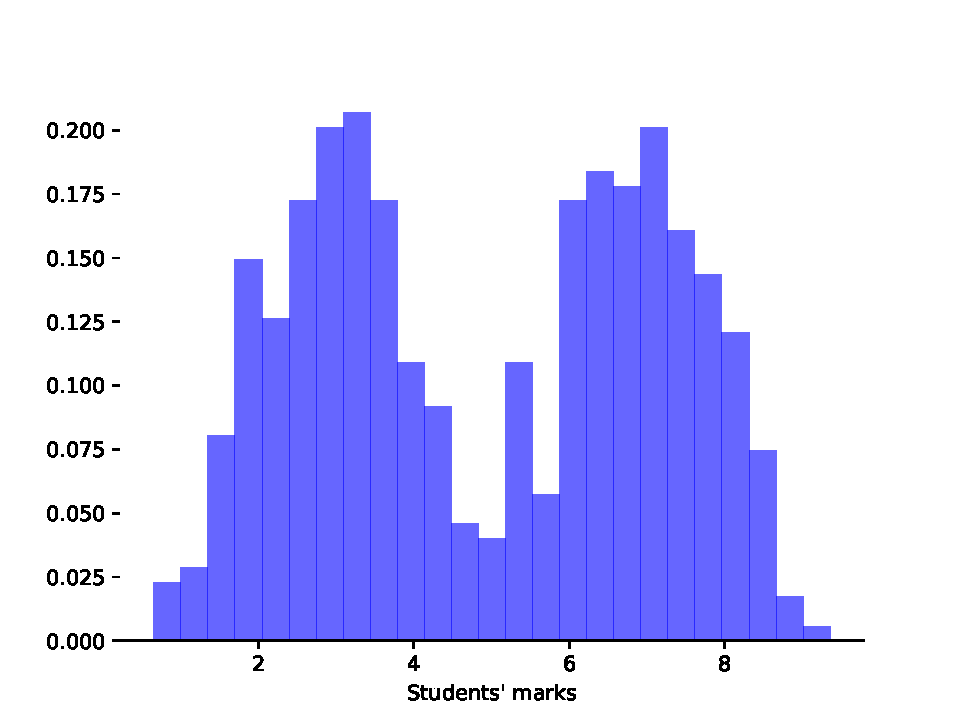
\includegraphics[width=\linewidth]{media/bimodal.pdf}
      \caption{Bimodal Distribution}\label{fig:linCM}
    \endminipage\hfill
    \minipage{0.45\textwidth}%
      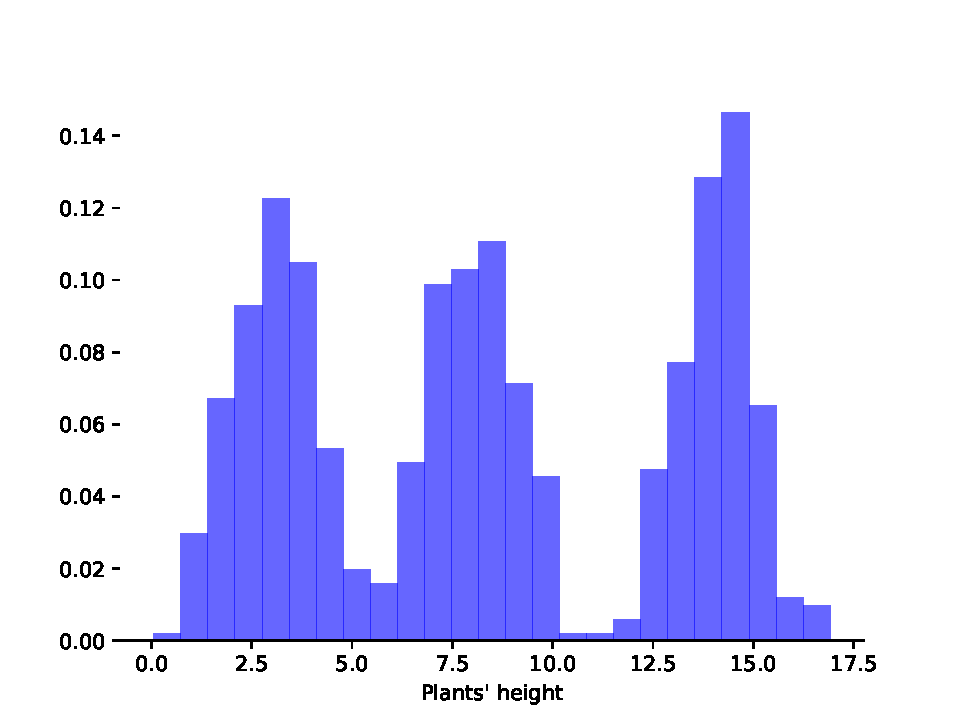
\includegraphics[width=\linewidth]{media/multimodal.pdf}
      \caption{Plants' height}\label{fig:RFCM}
    \endminipage
    \caption{Examples of bimodal and multimodal distributions.}
    \end{figure}
\end{nexample}


Now, given two distributions, we would like to determine how different they are from each other.
In order to compare them, we enunciate the definition of the Kullback-Leibler divergence.

\begin{ndefC}
Let $P$ and $Q$ be probability distributions over the same probability space $\Omega$. Then, the Kullback-Leibler divergence is defined as:
$$
D_{KL}(P \ || \ Q) = E_P\left[\log{\frac{P(x)}{Q(x)}}\right].
$$
\end{ndefC}
It is defined if, and only if, $P$ is \emph{absolutely continuous with respect to} $Q$, that is, if $P(A) = 0$ for any $A$ subset of $\Omega$ where $Q(A) = 0$.
 There are some properties of this definition that must be stated. 

\begin{nprop}
If $P,$ $Q$ are two probability distributions over the same probability space, then $D_{KL}(P|Q) \geq 0$.
\end{nprop}
\begin{proof}
Firstly, note that if $a \in \R^+$, then $\log \ a \leq a-1$. Then:
\begin{align*}
-D_{KL}(P \ || \ Q) & = - E_P\left[\log{\frac{P(x)}{Q(x)}}\right] \\
             & = E_P\left[\log{\frac{Q(x)}{P(x)}}\right] \\
             & \leq E_P\left[\left(\frac{Q(x)}{P(x)} - 1\right)\right]\\
             & = \int P(x) \frac{Q(x)}{P(x)} \mathop{dx} -1 \\
             & = 0.
\end{align*}
So we have obtained that $-D_{KL}(P\ ||\ Q) \leq 0$, which implies that $D_{KL}(P\ || \ Q) \geq 0$.
\end{proof}
As a corollary of this proposition, we can affirm that $D_{KL}(P\ ||\ Q)$ equals zero if and only if $P = Q$ almost everywhere. 
We will also remark the discrete case, as it will be used later. Let $P,Q$ be discrete probability distributions defined on the same probability space $\Omega$. Then, 
$$
D_{KL}(P\ ||\ Q) = \sum_{x \in \Omega} P(x) \log \left( \frac{P(x)}{Q(x)}\right).
$$

\section{Examples of distributions}

Let us present some examples o common distributions. They will be used further in this document.

\subsection{Bernoulli}

Think for a moment that you want to model the possible outcomes of an experiment with two possibilites: sucess or failure. Imagine also that you already know that in your experiment there is a probability $p$ of 
achieving success. That is the intuitive idea of a Bernoulli distribution. We can define it more formally as follows: 

The \emph{Bernoulli distribution} is a discrete probability distribution of a random variable that takes two values, $\{0,1\}$, with probabilities $p$ and $q = 1-p$, respectively. We will say that our distribution is a $Bern(p)$.

If $k$ is a possible outcome, we can define
the probability mass function $f$ of a Bernoulli distribution as:
$$
f(k,p) = 
\begin{cases} 
p, \quad & \text{ if } k=1,\\
1-p, \quad & \text{ if } k = 0.
\end{cases}
$$
Using the expression of the mean for discrete random variables, we obtain that $E[X] = p$ and 
$$
\Var[X] = E[X^2] - E[X]^2 = E[X] - E[X]^2 = p-p^2 = p(1-p) = pq.
$$

As a note, this is just a particular case of the \emph{Binomial distribution} with $n=1$.

\subsection{Gaussian Distribution}

The Gaussian (or normal) distribution is used to represent real-valued random variables whose distributions are not known.
Its importance relies in the fact that, using the \emph{central limit theorem}, we can assume that the average of many samples of
a random variable with finite mean and variance is a random variable whose distribution converges to a normal distribution as the number of samples increases.

\begin{ndef}
We say that the real valued random variable $X$ follows a \emph{normal distribution} of parameters $\mu,\sigma\in \R$ if, and only if,
its probability density function exists and it is determined by
\begin{equation}\label{gaussian:function}
f(x) = \frac{1}{\sigma \sqrt{2\pi}}e^{-\frac{1}{2}\left( \frac{x - \mu}{\sigma}\right)^2},
\end{equation}
where $\mu$ is the mean and $\sigma$ is its standard deviation. We denote this normal distribution as $X \sim \mathcal N (\mu,\sigma)$.
\end{ndef}

The particular case where $\mu = 0$ and $\sigma = 1$ is widely used in statistics. In this case, the density function is simpler:
\[
f(x) = \frac{1}{\sqrt{2\pi}}e^{-\frac{1}{2}x^2}.
\]

A remarkable property of these distributions is that, if $f : \R \to \R$ is a real-valued function defined 
as $f(x) = ax+b$, then $f(X) \sim \mathcal N (a\mu + b, \abs{a} \sigma)$.\\

In the same way that we extended random variables to random vectors, we can extend the normal distribution to a multivariate
random distribution.

\begin{ndef}
We say that a random vector $\bm{X} = (X_1,\dots,X_n)$ follows a multivariate normal distributions of parameters
$\mu \in \R^n$, $\Sigma \in \mathcal M_N(\R)$ if, and only if, its probabity density function is:
\begin{equation*}\label{gaussian:function:vector}
f(x) = \frac{1}{\sqrt{\det(2\pi \Sigma)}}e^{-\frac{1}{2}(x - \mu )^T \Sigma^{-1} (x-\mu)}.
\end{equation*}
It is denoted $X \sim \mathcal N(\mu, \Sigma)$.
In this case, $\mu$ is the mean vector of the distribution and $\Sigma$ denotes the covariance matrix.  
\end{ndef}



\clearpage

\ctparttext{
  \color{black}
  \begin{center}
  Information theory is the base for all the following work. In this part, \emph{Mutual Information} will be explained and then, bounds for this function will be given.
  \end{center}
}
\part{Information Theory}
\chapter{Mutual Information}
Obtaining good representations of data is one of the most important tasks in machine learning (ML). 
Recently, it has been discovered that maximizing \emph{mutual information} between two elements in our data can give us good representations for our data.
In this section, \emph{information theory} notions will be presented, in order to use them in our ML models. This will provide a theoretical solid base for
the notions explained later.



\section{Entropy}

The \emph{mutual information} concept is based on the \emph{Shannon entropy}, which we will introduce first, along with some basic properties of it. The Shannon entropy is a way of measuring the uncertainty in a random variable. 
Given an event $\mathcal A \in \Alg$, $P$ a probability measure and $P[\A]$ the probability of $\mathcal A$, we can affirm that 
$$
\log\frac{1}{P[\mathcal A]}
$$
describes \emph{"how surprising is that $\A$ occurs"}. For instance, if $P[\A] = 1$, then the last expression is zero, which means that it is not a surprise that $\A$ occurred. With this motivation, we get to the following definition.


\begin{ndef}
Let $X$ be a discrete random variable with image $\X$. The \emph{Shannon entropy}, or simply \emph{entropy}  $H(X)$ of $X$ is defined as:
$$
H(X) = E_X\left[\log\frac{1}{P_X(X)}\right] =  \sum_{x \in \X} P_X(x) \log\frac{1}{P_X(x)}.
$$
\end{ndef}
The \emph{entropy} can trivially be expressed as:
$$
H(X) = - \sum_{x \in \X}P_X (x)\log P_X(x).
$$

The simple example, \citep{cover_elements_1991}, even though it is very simple, it is very illustrative for our definition:

%http://www.cs.columbia.edu/~vh/courses/LexicalSemantics/Association/Cover&Thomas-Ch2.pdf
\begin{nexample}
    \label{example:entropy}
Let $X \sim Bern(p)$. Then, the entropy of $X$ is:
\[
H(X) = -p \log p - (1-p) \log(1-p)) = H(p),
\]
since $H$ only depends on $p$. In Fig. \ref{fig:example:entropy} we can see a representation of this function. We appreciate that in this case, $H$ is concave and equals $0$ if $p \in \{0,1\}$, which are the values of $p$ that give us no uncertainty. The maximum uncertainty is obtained when $p=\frac{1}{2}$, where we do not know what to expect as an outcome from our random variable $X$.

\begin{figure}[H]
    \label{fig:example:entropy}
    \centering
    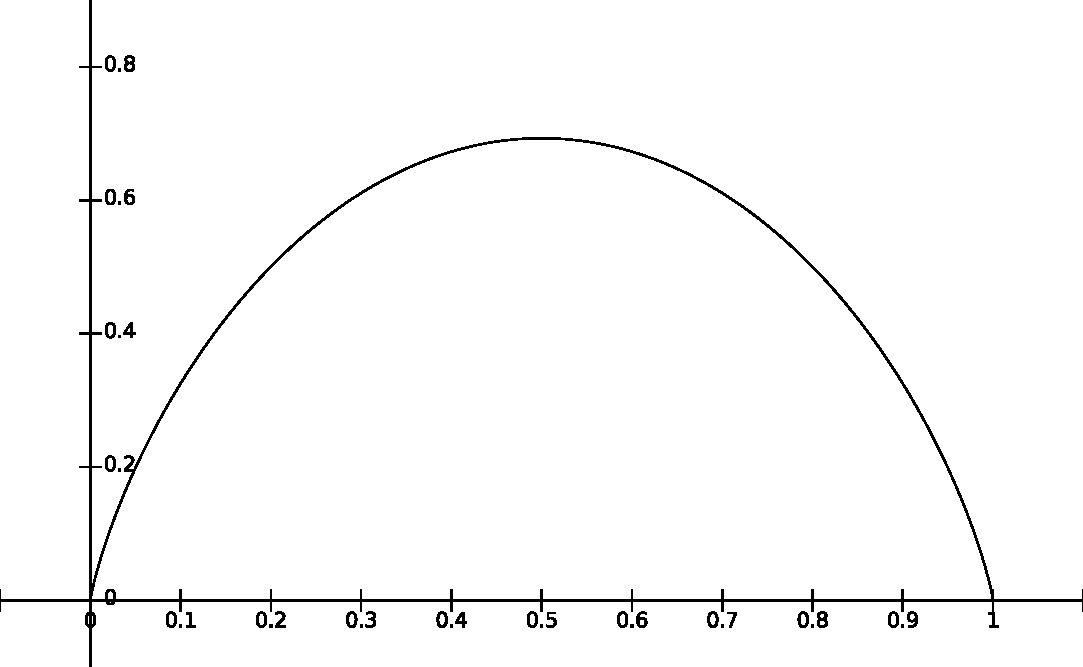
\includegraphics[scale=0.4]{Entropy.pdf}

      \caption{Representation of $H(p)$ in the example \ref{example:entropy}.}
\end{figure}

\end{nexample}


It can also be proven that, in general, the entropy is concave. There are some properties of the \emph{entropy} that must be remarked. 
\begin{nprop}\label{entr:prop:1}
    Let $X$ be a random variable with image $\X$. If $|\X|$ is the cardinal of $\X$, then
    $$
0 \leq H(X) \leq \log(|\X|).
    $$
\end{nprop}
\begin{proof}
    Since $\log y$ is concave on $\R^+$, by Jensen's inequality ( see Appendix A, Prop. \ref{prop:jensen}), we obtain:
    $$
    H(X) = - \sum_{x \in \X}P_X (x)\log P_X(x) \leq \log\left(\sum_{x \in \X} 1\right) = \log(|\X|).
    $$
    For the lower bound we see that, since $P_X(x) \in [0,1]$ for all  $x \in \X $ then $\log P_X(x) \leq 0 \ \ \forall x \in \X$. Hence , $-P_X(x) \log P_X(x) \geq 0$ for all $x \in X$, so $H(X) \geq 0$.
\end{proof}
We can also see that the equality on the left holds if , and only if , exists $ x $ in  $X$ such that its probability is exactly one, that is $P_X(x) = 1$. The right equality holds if and only if , for all $x \in \X$, its probability is $P_X(x) = \frac{1}{\abs{X}}$.

\subsection*{Conditional entropy}
We have already said that entropy measures how surprising is that an event occurs.
Usually, we will be looking at two random variables and it would be interesting to see how likely is that one of them, say $X(x)$, occurred, if we already know that $Y(y)$ occurred. 
This leads us to the definition of \emph{conditional entropy}. Let us see a simpler case first:

Let $A$ be an event, and $X$ a random variable. The conditional probability $P_{X|A}$ defines the entropy of $X$ conditioned to $ A$:
$$
H(X| A) = \sum_{x \in \X} P_{X|A}(x) \log\frac{1}{P_{X|A}(x)}.
$$
If $Y$ is another random variable and $\mathcal Y$ is its image, intuitively we can sum the conditional entropy of an event with all the events in $\mathcal Y$, and this way we obtain the conditional entropy of $X$ given $Y$.
\begin{ndef}[Conditional Entropy]
Let $X,Y$ be random variables with images $\X,\mathcal Y$. The \emph{conditional entropy} $H(X | Y)$ is defined as:

\begin{equation*}
    \begin{split}
    H(X|Y) &  :=   \sum_{y \in \mathcal Y} P_{\mathcal Y}(y) H(X| Y = y)  \\ 
    & = \sum_{y \in \mathcal Y} P_{\mathcal  Y}(y) \sum_{x \in \X} P_{X | Y}(x|y)\log\frac{1}{P_{X|Y}(x|y)}  \\
   & = \sum_{x \in X,y \in \mathcal Y}P_{XY}(x,y)\log\frac{P_Y(y)}{P_{XY}(x,y)}.
\end{split}
\end{equation*}
\end{ndef}

The interpretation of the conditional entropy is simple: the uncertainty in $X$ when $Y$ is given.
Since we know about an event that has occurred ($Y$), intuitively the conditional entropy , or the uncertainty of $X$ occurring given that $Y$ has occurred, will be lesser than the entropy of $X$, since we already have some information about what is happening. We can prove this:

\begin{nprop}\label{entr:prop:2}
Let $X,Y$ be random variables with images $\mathcal X, \mathcal Y$. Then:
$$
0 \leq H(X|Y) \leq H(X).
$$
\end{nprop}
\begin{proof}

The inequality on the left was proved on Proposition \ref{entr:prop:1}. The characterization of when $H(X|Y) = 0$ was also mentioned after it.
Let us look at the inequality on the right. Note that restricting to the $(x,y)$ where $P_{XY}(x,y) > 0$ and using the definition of the conditional probability we have:
\begin{align*}
H(X|Y) = & \sum_{y \in \mathcal{Y}} P_Y(y) \sum_{x \in \X} P_{X|Y}(x|y)\log \frac{1}{P_{X|Y}(x|y)}\\
 = & \sum_{x \in \mathcal X,y \in \mathcal Y} P_Y(y) P_{X|Y}(x,y) \log \frac{P_Y(y)}{P_{XY}(x,y)} \\
  = & \sum_{x \in \mathcal X,y \in \mathcal Y} P_{XY}(x,y)\log \frac{P_Y(y)}{P_{XY}(x,y)} ,
\end{align*}
and 
$$
H(X) = \sum_x P_X(x) \log \frac{1}{P_X(x)} = \sum_{x,y}P_{XY}(x,y) \log \frac{1}{P_X(x)}.
$$
Hence,
\begin{equation}\label{eq:dif-expr-mi}
\begin{split}
H(X|Y) - H(X) = & \sum_{x,y}P_{XY}(x,y) \left( \log \frac{P_Y(y)}{P_{XY}(x,y)} - \log \frac{1}{P_X(x)}\right) \\ 
= &  \sum_{x,y}P_{XY}\log \frac{P_Y(y)P_X(x)}{P_{XY}(x,y)}.
\end{split}
\end{equation}
So, using Jensen's inequality, we obtain:
\begin{align*}
\sum_{x,y}P_{XY}\log \frac{P_Y(y)P_X(x)}{P_{XY}(x,y)} \leq & \log \left( \sum_{x,y}\frac{ \cancel{P_{XY}(x,y)} \ \  P_Y(y) P_X(x)}{\cancel{P_{XY}(x,y)}} \right) \\ 
= & \log\left( \left( \sum_x P_X(x) \right) \left(\sum_y P_Y(y)\right)\right) = \log 1 = 0,
\end{align*}
and this leads us to:
\begin{equation}\label{prop:2:2nd:ineq}
H(X|Y) - H(X) \leq 0 \quad \text{ then } \quad H(X|Y) \leq H(X)
\end{equation}
as we wanted.
\end{proof}

It must be noted that the inequality the state of the proposition,
$$
0 \leq H(X|Y) \leq H(X),
$$

in the inequality of the left, equality holds if, and only if, $P_{XY}(x,y) = P_X(x) P_Y(y)$ for all $(x,y)$ with $P_{XY} (x,y) > 0$, as it is said in Jensen's inequality.
For the inequality on the right, equality holds if and only if $P_{XY}(x,y) = 0$, which implies $P_X(x)P_Y(y) = 0$ for any $x\in \mathcal X$, $y \in \mathcal Y$. It follows that $H(X|Y) = H(X)$ if and only if $P_{XY}(x,y) = P_X(x)P_Y(y)$ for all $(x,y) \in \mathcal X \times \mathcal Y$


\section{Mutual Information}

Using the entropy of a random variable we can directly state the definition of \emph{mutual information} as follows:

\begin{ndef}
Let $X,Z$ be random variables. The \emph{mutual information (MI)} between $X$ and $Z$ is expressed as the difference between the entropy of $X$ and the conditional entropy of $X$ and $Z$, that is:
$$
I(X,Z) := H(X) - H(X|Z).
$$
\end{ndef}

Since the entropy of the random variable $H(X)$ explains the uncertainty of $X$ occurring, the intuitive idea of the \emph{MI} is to determine the decrease of uncertainty of $X$ occurring when we already
know that $Z$ has occurred. We also have to note that, using the definition of the \emph{entropy} and the expression obtained in Eq. \ref{eq:dif-expr-mi}, we can rewrite the \emph{MI}  it follows:
\begin{align*}
I(X,Z) & = \sum_{x \in \X}P_X(x) \log \frac{1}{P(x)} - \sum_{x \in \X, z \in \mathcal Z} P_{XZ}(x,z) \log \frac{P_Z(x)}{P_{XZ}(x,z)} \\  & = \sum_{x,z}P_{XZ}\log \frac{P_Z(z)P_X(x)}{P_{XZ}(x,z)} = D_{KL}(P_{XZ} \ || \ P_X P_Z)
\end{align*}
and we have obtained an expression of the mutual information using the \emph{Kullback-Leibler} divergence. This provides with the following immediate consequences:
\begin{enumerate}[label=$(\roman*)$]
\item Mutual information is non-negative. That is : $I(X,Z) \geq 0$.
\item If $X,Z$ are random variables, then its mutual information equals zero if, and only if, they are independent. 
This easy to check since if $D_{KL}(P_{XZ} \ || \ P_X P_Z) = 0$, then $P_{XZ} = P_X P_Z$ almost everywhere so $X$ and $Z$ are independent.p
\item Since $P_{XZ} = P_{ZX}$ and $P_X P_Z = P_Z P_X$, mutual information is symmetric. That is: $I(X,Z) = I(Z,X)$.
\end{enumerate}

\begin{remark} We can set a connection between the mutual information and sufficient statistics. Let $T(X)$ be a statistic. We say that $T(X)$  is sufficient for $\theta$ if its mutual information with $\theta$ equals the mutual information between $X$ and $\theta$, that is:
$$
I(\theta, X) = I (\theta, T(X)).
$$
This means that sufficient statistics preserve mutual information and conversely.
\end{remark}

\clearpage

\ctparttext{
  \color{black}
  \begin{center}
  Clarification of this part
  \end{center}
}
\part{Representation Learning}
\chapter{Context}
\label{Chapter:Intro:Rep:Learning}

\emph{Machine learning} is the field of computer science that studies algorithms that improve automatically through experience from examples. 
These algorithms allow computers to discover how to
perform tasks without being explicitly programmed to do them. For the computers to learn, it is mandatory that a finite set of data (or dataset) $\D$ is available. 

Whenever a computer is providen with data, the data can be \emph{labeled} or \emph{unlabeled}. Labeled data is the one that, each point $x_i \in \D$ is related to a tag $y_i \in Y$, where $Y$ is a set of classes.
Unlabeled data is the kind of data that does not have a label or class associated to it, so it is just $x_i \in \R^d$. 

Depending on how the data (\emph{or signal}) is given to the computer, the machine learning approaches can be divided into three broad categories:
\begin{enumerate}
    \item \emph{Supervised learning}. In this category the goal is to use the labeled data in order to find a function that maps the dataset to the set of classes. That is a function $g:\D \to Y$. 
    An example of supervised learning is image classification: giving a label to an image.
    \item \emph{Unsupervised learning}. In ths case, the data is unlabeled, so the approach is completely different. Usually, the goal here is to discover hidden patterns in data or to learn features from it.
    An example of this kind of learning is K means, which consistis in clustering the data in $k$ groups. It is also known as \emph{self-supervised} learning.
    \item \emph{Reinforcement learning}. This is the area concerned with how intelligent agents take decisions in a specific environment in order to obtain the best reward in their objective. It focuses on finding a balance between exploration of uncharted territory and explotation of the current knowledge.

\end{enumerate}

In this work, we will focus on unsupervised learning. Particularly, in representation learning.

There are many different tasks that can be performed with the data, such as linear regression, logistic regression, or classification. In any of these tasks, computers might need
to do intermediate steps before giving a label to the input example. Sometimes, they must create a \emph{representation} that 
contains the data's key qualities.  Here is where \emph{representation learning} is born. 


Having a representation $\tilde{x}$ of a datapoint $x\in \R^d$, if a machine learning model
tries to make a posterior task, such as classification, the input $x$ must be transformed to a, usually lower dimensional, vector $r$ in order to perform the final label.

\emph{Features} are parts or patterns of an datapoint $x \in \D$ that help to identify it. In fact, it is desiderable that this attribute is shared by all independent units that represent the same object. For instance, if we consider an image of any square, we should be able to identify 4 corners and 4 edges. These could be features of a square.
When we mention feature detection, we are adressing the methods for detecting these features of a datapoint.

Representation learning is a set of techniques that allow a system to discover the representations needed for feature detection or classification. 
In contrast to manual feature engineering (which involves manually exploring the data and finding relationships in it), feature learning allows a machine to learn the features and to use them to perform a task.\\

Feature learning can be supervised or unsupervised. 
\begin{itemize}
    \item In supervised feature learning, representations are learned using labeled data.Examples of this kind of feature learning are supervised neural networks and multilayer perceptron. 
    \item In unsupervised learning, the features are learned using unlabeled data. There are many examples of this, such as independent component analysis (ICP) and autoencoders.
\end{itemize}
 In this work, we will be working with unsupervised feature learning, so we will have unlabeled data that we would like to find a representation for.


The performance of machine learning methods is heavily dependent on the choice of data features \citep{bengio_representation_2014}. This is why most of the current 
effort in machine learning focuses on designing preprocessing and data transformation that lead to good quality representations. A representation will be of good quality when its features
produce good results when we evaluate the \emph{accuracy} of our model.\\

The main goal in representation learning is to obtain features of the data that are generally good for either of the supervised tasks. These tasks are usually called \emph{downstream tasks}. That is, we would like to obtain
a representation that is either good for image classification (giving an image a label of what we can see in it) or image captioning (producing a text that describes the image).

Data's features that are invariant through time are very useful for machine learning models. In \citep{wiskott_slow_2002}, \emph{slow features} are presented. Slow features are defined as features of a signal 
(which can be the input of a model) that vary slowly during time. That means, if $\bm{X}$ is a \emph{time series}\footnotemark, we will try to find any number of features in $\bm{X}$ that vary the most slowly.
These kind of features are the most interesting ones when creating representations, since they give an abstract view of the original data.\\


%------------- Footnotemark
\footnotetext{A time series is an ordered sequence of values of a random variable at, usually, equally spaced time intervals.}
%----------------------

\begin{nexample} In computer vision, the value of the pixels in an image can vary fast. For instance, if we have a zebra on a video and the zebra is moving from one side of the image to the other, due 
to the black stripes of this animal, the pixels will fast change from black to white and viceversa, so value of pixels is probably not a good feature to choose as an slow feature. However, there will always
be a zebra on the image, so the feature that indicates that there is a zebra on the image will stay positive throughout all the video, so we can say that this is a slow feature.
\end{nexample}

We will be studying different models that try to learn representations from raw data without labels, as we have mentioned. We usually need a function that measures what is the penalty that the model gets for a choice of a parameter.
This is called a \emph{loss function}, that we will want to optimize.

For instance, in a regression problem, a good example of loss function is \emph{mean squared error}, which is expressed as follows:
\[
\text{MSE} = \frac{\sum_{i =1 }^n \left(y_i - \hat{y_i}\right)^2}{n}.
\]
In a classification problem, each datapoint $x_i$ has a correct classification $y_i$. In this case, the score of the correct category $y_i$ should be greater than the sum of the scores of all incorrect categories $y_j$ with $j \neq i$,
 so we could use a function like \emph{support vector machine (SVM) loss}:
\[
\text{SVMLoss} = \sum_{j \neq y_i} \max(0,s_j - s_{y_i} + 1)
\]


In the context of machine learning, a \emph{model} is the result of running a maching learning algorithm in data. This model will represent what the computer has learned from the data using this algorithm. As an easy example, when we use a
linear regression algorithm, we obtain a model that is a vector of coefficients with specific values.

In the following chapters, we will explain different kinds of neural networks and which kind of loss functions they use. 

\clearpage
\chapter{Generative Models}
From now on, let $\D$ be any kind of observed data. This will always be a finite subset of samples taken from a probability distribution $\pd$. There are models that, given $\D$, try to approximate the 
probability distribution that lies underneath it. These are called \emph{generative models (G.M.)}. 

Generative models can give parametric and non parametric approximations to the distribution $\pd$. 
In our case, we will focus on parametric approximations where the model searches for the parameters that minimize a chosen metric (which can be a distance or other kind of metric such as K-L divergence) between the model distribution and the data distribution. 

We can express our problem more formally as follows. Let $\theta$ be a generative model within a model family $\mathcal M$. The goal of generative models is to optimize:
$$
\min_{\theta \in \mathcal M} d(\pd,p_\theta),
$$
where $d$ stands for the distance between the distributions. We can use, for instance, K-L divergence.

Generative models have many useful applications. We can however remark the tasks that we would like our generative model to be able to do. Those are:
\begin{itemize}
\item Estimate the density function: given a datapoint, $x \in D$, estimate the probability of that point $p_\theta(x)$.
\item Generate new samples from the model distribution $x \sim p_\theta(x)$.
\item Learn useful features of the datapoints.
\end{itemize}

If we have a look again at the example of the zebras, if we make our generative model learn about images of zebras, we will expect our $p_\theta(x)$ to be high for zebra's images. We will also expect the model
to generate new images of this animal and to learn different features of the animal, such as their big size in comparison with cats.

\section{Autoregressive Models}

A very first definition of \emph{autoregressive models (AR)} would be the following one: \emph{autoregressive models are feed-forward models that predict future values using past values}. Let us go deeper into this 
concept and explain how it behaves.

Again, let $\D$ be a set of $n-$dimensional datapoints $x$. We can assume that $x \in \{0,1\}^n$ for simplicity, without losing generality. If we choose any $x\in \D$, using the chain rule of probability, we obtain
$$
p(x) = \prod_{i=1} ^n p(x_i | x_1,\dots,x_{i-1}) = \prod_{i = 1}^n p(x_i|\bm{x}_{<i}), \quad  \text{ where }  \quad \bm{x}_{<i} = [x_1,\dots, x_{i-1}].
$$
We see using that expression how, fixing an order of the variables $x_1,\dots,x_n$, the distribution for the $i$-th random variable depends on all the preceding values in the particular chosen order. 

It is known that given a set of discrete and mutually dependent random variables, they can be displayed in a table of conditional probabilities. If $K_i$ is the number of states that each random variable can take
then $\prod K_i$ is the number of cells that the table will have. If we represent $p(x_i|\bm{x}_{<i})$ for every $i$ in tabular form, we can represent
any possible distribution over $n$ random variables. 

This, however, will cause an exponential growth on the complexity of the representation, because in our case we would need to specify $2^{n-1}$ possibilities 
for each case. In terms of neural networks, since each column must sum $1$ because we are working with probabilities, we have $2^{n-1}-1$ parameters for this conditional, and the tabular representation
becomes impractical for our network to learn.

In autoregressive generative models, the conditionals are specified as we have mentioned before: parameterized functions with a fixed numbers of parameters. More precisely,  we assume 
the conditional distributions to be Bernoulli random variables and learn a function $p_{\theta_i}$ that maps these random variables to the mean of the distribution. Mathematically, we have to find 
$$
p_{\theta_i}(x_i | \bm{x}_{<i}) = Bern(f_i(x_1,\dots,x_{i-1})),
$$
where $\theta_i$ is the set of parameters that specify the mean function $f_i:\{0,1\}^{i-i} \to [0,1]$.

The number of parameters is then reduced to $\sum_{i=1}^n \abs{\theta_i}$, and then we can not represent all possible distributions as we could when using the tabular form of the conditional probabilities.
We are now setting the limit of its expressiveness because we are setting the conditional distributions $p_{\theta_i}(x_i|\bm{x}_{<i})$ to be \emph{Bernoulli} random variables. 

Let us see a very simple case first in order to understand it better and then we will generalize it. Let $\sigma$ be a sigmoid non linear function and 
$\theta_i = \{\alpha_{0}^{(i)},\alpha_{1}^{(i)},\dots, \alpha_{i-1}^{(i)}\}$ the parameters of the mean function. Then, we can define our function $f_i$ as the application of the non linear function to the
sum of the first parameter $\alpha_0^{(i)}$ with the product of each parameter $\alpha_{j}^{(i)}$ with its random variable $x_j$, with $j =1,2,\dots,i-1$ .  That is:
$$
f_i(x_1,\dot, x_{i-1}) = \sigma(\alpha_{0}^{(i)} + \alpha_{1}^{(i)}x_i + \dots + \alpha_{i-1}^{(i)}x_{i-1}).
$$
In this case, the number of parameters would be $\sum_{i = 1}^n i = \frac{n(n+1)}{2}$, so using \emph{Big }$O$ notation, we would be in the case of $O(n^2)$. We will state now a more general and useful case,
giving a more interesting parametrization for the mean function: \emph{multi layer perceptrons}\footnotemark (MLP).

%------------- Footnotemark
\footnotetext{Multi layer perceptrons are feed-forward neural networks with at least 3 layers: input, hidden and output layers; each one using an activation
function.}
%----------------------

For this example we will consider the most simple MLP: the one with one hidden layer. Let $h_i = \sigma(\bm{A}_i \bm{x}_{<i} + c_i)$ be the hidden layer activation function. Remember that $h_i \in \R^d$. Let
$ \theta_i = \{ \bm{A}_i \in \R^{d \times (i-1)}, \ c_i \in \R^d, \ \alpha^{(i)} \in \R^d, \ b_i \in \R\}$ the set of parameters
for the mean function $f_i$, that we define as:
$$
f_i(\bm{x}_{<i}) = \sigma(\alpha^{(i)}h_i + b_i)
$$
In this case, the number of parameters will be $O(n^2 d)$.

\chapter{Contrastive Predictive Coding}
We are now ready to connnect the concepts of mutual information and generative models that we have presented. In unsupervised learning,
it is a common strategy to predict future information and to try to find out if our predictions are correct.
In \emph{natural language processing},for instance, representations are learned 
using neighbouring words (https://arxiv.org/pdf/1301.3781.pdf), and in images, some studies have been able to predict color from grey-scale (https://arxiv.org/pdf/1505.05192.pdf).

When we talk about high-dimensional data, it is not useful to make use of an unimodal loss function to evaluate our model. If we did it like this, we would be assuming that there is only
one peak in the distribution function and that it is actually similar to a Gaussian.  This is not always true, so we can not assume it for our models. Generative models can be used for this purpose:
they will model the relationships in the data $x$. However,they ignore the context $c$ in which the data $x$ is involved. As an easy example of this, an image contains thousands of bits of information,
while the label that classifies the image contains much less information , say, $10$ bits for $1024$ categories. Because of this, modeling $p(x|c)$ might not be the best way to proceed if we want
to obtain the real distribution that generates our data. 

Our goal here will be to seek for a way of extracting shared information between the context and the data. Due to the differences in data dimensionality, if we want to predict the future $x$ using the context $c$, firstly we must
encode our entry data $x$ into a representation which size is comparable to context size. Firstly, an \emph{encoder} is used. An encoder is a model that, given an input $x$, provides a feature map or vector that holds the information
that the input $x$ had. In fact, and here is where we link the mutual information with the current topic, we want our encoder to maximize
$$
I(x,c) = \sum{x,c}p(x,c)\log\frac{p(x|c)}{p(x)}
$$
that is, the mutual information between the input $x$ and the context $c$.  Maximizing the mutual information between $x$ and $c$, we extract the latent variables
that the inputs have in common.

So, we will use an encoder $g_{enc}$ that transforms the input sequence of observations $x_t$ to a sequence of latent representations
$$
z_t = g_{enc}(x_t).
$$
After we have obtained $z_t$, we use it as input of an autoregressive model to produce a context latent representation:
$$
c_t = g_{ar}(z_{\leq t}).
$$
In this case, $c_t$ will summarize the information of $z_i$ for $i \leq t$. Following the argument that we gave before, predicting the future $x_{t+k}$ using only a generative model, say $p_k(x_{t+k}|c)$
might not be correct, since we would be ignoring the context.


\clearpage 

\ctparttext{
  \color{red}
  \begin{center}
    Appendices
  \end{center}
}
\part{APPENDIX A}
\label{APPENDIX:A}

This appendix will be used to set forth some theoretical results that might not always be relevant but are needed to understand some details during this thesis. Not all of them will be proven.

\begin{nprop}[Jensen's Inequality]\label{prop:jensen}
    Let $f:\mathcal D \to \R$ be a concave function and $n\in \mathbb N$. For any $p_1,\dots,p_n \in \R^+_0$ with $\sum p_i = 1$ and any $x_1,\dots,x_n \in \mathcal D$, it holds that:
    $$
    \sum_{i = 1}^n p_i f(x_i) \leq f \left(\sum_{i=1}^n p_i x_i\right).
    $$
    Furthermore, if $f$ is \emph{strictly} concave and $p_i \geq 0$ for all $i  = 1,\dots,n$, then the equality holds if, and only if, $x_1 = \dots = x_n$.
\end{nprop}

In Chapter \ref{Chapter:connection:triplets}, the norm $\norm{\cdot}_2$ is mentioned. Norm theory is a very extense field, so we will only mention the definition and the norm that we will use in the text.

\begin{ndef}\label{def:norm}
Given a vector space $X$ over a subfield $F$ of the complex numbers $\mathbb C$, a \emph{norm} is a real valued function $\norm{\cdot}:X \to \R$ with the following properties:
\begin{enumerate}
\item Triangle inequality, that is: $\norm{x+y} \leq \norm{x} + \norm{y}$ for all $x,y \in X$.
\item Absolute homogeinity, that is: $\norm{sx} = \abs{s}\norm{x}$ for all $x\in X$ and any scalar $s$.
\item Positive definiteness, that is $\norm{x} \geq 0 $ for all $x \in X$ and $\norm{x} = 0$ if, and only if, $x = 0$.
\end{enumerate}
\end{ndef}
In particular, the $\norm{\cdot}_2$ that we used in the euclidean space $\R^n$, is defined as follows:
\[
\norm{x}_2 := \left(\sum_{i = 1}^n x_i^2\right)^{\frac{1}{2}}, \quad \quad \forall x \in \R^n.     
\]



\nocite{*}
\bibliographystyle{authordate1}
\bibliography{Bibliography}

\end{document}
